\documentclass[11pt]{article}
\usepackage[margin=1in,letterpaper]{geometry}
\usepackage{times}
\usepackage{amsmath,amssymb,amsthm}
\usepackage{graphicx}
\usepackage{booktabs}
\usepackage[round,authoryear]{natbib}
\usepackage{hyperref}
\usepackage{caption}
\usepackage{setspace}
\usepackage{microtype}
\usepackage{xcolor}
\usepackage{enumitem}

\hypersetup{colorlinks=true, linkcolor=blue!50!black, citecolor=blue!50!black, urlcolor=blue!50!black}

\setlength{\parskip}{0pt}
\setlength{\parindent}{20pt}
\renewcommand{\arraystretch}{1.1}
\captionsetup{font=small,labelfont=bf,labelsep=period,skip=4pt}

\newtheorem{proposition}{Proposition}
\newtheorem{lemma}{Lemma}

\title{Late, Rare, and Suboptimal:\\
A Real-Options Analysis of\\
NHL Coaches' Timeout Decisions}

\author{}
\date{}

\begin{document}

\maketitle
\thispagestyle{empty}

\begin{abstract}
\noindent NHL rules grant each team a single thirty-second timeout per regulation game. The decision-theoretic structure of this rule is that of a one-shot real option held by the coaching staff that expires worthless when regulation ends. Using the official NHL Web API for the 2022--2023 through 2024--2025 regular seasons, we assemble a corpus of 3{,}936 games, 1{,}242{,}481 plays, and 468 verified timeout events. Three empirical facts dominate the data: 94.05 percent of team-games end with the timeout unused; the median call lands at minute 58.5 of regulation; and two-thirds of calls coincide with a calling-team skater advantage, consistent with pulled-goalie offensive setups. We solve the calling team's optimal-stopping problem by backward induction on a thirty-second time grid using the empirical league goal-arrival rate, and sweep the timeout-boost parameter $\mu \in \{0.005, 0.01, 0.02, 0.03\}$. The implied optimal policy uses the timeout in 58 to 86 percent of team-games at a median call eight to eleven minutes earlier than current practice. The dominant component of the divergence is call frequency, not call timing: the option-decay term in the Bellman equation is being ignored. The pattern survives a state-dependent boost amplifying the pulled-goalie scenario, sensitivity to the league scoring rate, and an asymmetric scoring-rate specification that incorporates score effects. We estimate the EU loss at 0.0014 to 0.0043 win-probability points per team-game, accumulating to roughly 3.7 wins per season league-wide.

\noindent\textbf{Keywords:} hockey analytics; optimal stopping; real options; win probability; coaching decisions; expected utility.
\end{abstract}

\onehalfspacing

\section{Introduction}

The choice of whether and when to call a timeout is one of the few discrete in-game tactical decisions in NHL hockey that a coach controls unilaterally. Each team is allotted exactly one thirty-second timeout per regulation game. The team may call it at any whistle in regulation or overtime, and any unused portion lapses without effect when regulation ends. The decision-theoretic structure is that of a single-exercise real option \citep{DixitPindyck1994}: the coaching staff holds a one-shot right whose underlying value depends on game state at exercise, and whose terminal value is zero.

The conventional NHL coaching rule of thumb reserves the timeout for late-game high-leverage situations: a critical defensive-zone faceoff trailing by one goal in the final minute, or an offensive-zone faceoff after a stoppage with the goaltender pulled. Across the three regular seasons we examine (2022--2023 through 2024--2025), 73.5 percent of all timeouts are called in the third period and 62.6 percent fall within the final five minutes of regulation. The median call lands at minute 58.5, ninety seconds before the regulation buzzer.

The puzzle this paper addresses is whether such uniformity reflects optimal play. There are two reasons for skepticism. First, the unconditional probability that a team reaches a high-leverage tied-or-one-goal late-third-period state is bounded well below one. With probability roughly 0.94 per team-game the canonical-target state never arrives, and the timeout expires unused. The option-decay term in any Bellman recursion of the coach's problem is therefore large. Second, alternative high-leverage states exist earlier in regulation: a tied score with seven minutes remaining, a one-goal deficit on a power play in the second period, a defensive-zone faceoff after an opponent icing while shorthanded. A coach who reserves the option for the strict global maximum of state-leverage will routinely pass over local maxima reached with higher unconditional probability.

This paper formalizes the timeout decision as an optimal-stopping problem and solves it numerically using empirically-calibrated league scoring dynamics. We then compare the implied optimal exercise distribution to the observed distribution. The optimal policy uses the timeout in 58 to 86 percent of team-games depending on the assumed boost parameter, against an observed rate of 5.95 percent. The optimal median call time precedes the observed median by eight to eleven minutes. The optimal calling region opens at score differentials $d \in \{-1, 0, +1\}$ at minute 48 to 50; observed calls cluster eight minutes later. The misalignment is one-sided: NHL coaches do not over-use timeouts in any region of the state space, and they do not call timeouts too early.

The closest methodological precedent is the pulling-the-goalie literature \citep{BeaudoinSwartz2010, Asmussen2011}. That literature established that NHL coaches waited too long to pull goalies trailing late in regulation, and the formally-optimal threshold sits at 2.5 to 3 minutes remaining trailing by one rather than the conventional sub-one-minute mark. The empirical effect has been observable: the median pull time in the NHL has migrated earlier by about ninety seconds over the past decade. The timeout-timing literature stands at a similar pre-revision stage today, with one structural difference. The timeout has zero terminal salvage value, while a pulled goalie still produces some shot attempts. The option-decay term that drives the central result here is therefore sharper than in the goalie problem.

\subsection{Contribution}

We make three contributions. First, we document the underuse of NHL timeouts using the post-2022 official play-by-play feed, finding a 5.95 percent per-team-game usage rate substantially below the figure in the closest precursor study \citep{Ferer2020} and consistent with a continued decline over the last decade. Second, we provide a formal real-options model of the timeout decision and solve it numerically, producing the first explicit optimal-stopping threshold for NHL timeouts in the published literature. Third, we show that the magnitude of the empirical-optimal gap is robust across a wide range of timeout-boost parameters, scoring-rate calibrations, terminal conditions, and a state-dependent boost specification that handles the pulled-goalie scenario explicitly. Even under the most conservative parameterization the gap exceeds an order of magnitude in usage rate. The boost parameter would have to fall to economically implausible levels for current practice to be EU-rationalizable.

The remainder of the paper is organized as follows. Section~\ref{sec:lit} reviews the related literature on coaching decision-making, hockey analytics, and the optimal-stopping foundations. Section~\ref{sec:theory} sets up the formal model. Section~\ref{sec:data} describes the data and the verification protocol. Section~\ref{sec:empirics} presents the empirical patterns of use. Section~\ref{sec:numerical} solves the optimal-stopping problem and compares the implied and observed distributions. Section~\ref{sec:robustness} reports the robustness battery. Section~\ref{sec:discussion} discusses competing explanations, the methodological parallel to the pulling-the-goalie literature, and the practical implications for NHL coaching staffs.

\section{Related Literature}\label{sec:lit}

This paper sits at the intersection of three literatures: the empirical study of suboptimality in professional sports coaching, the methodological tradition of in-game win-probability estimation, and the optimal-stopping foundations of real-options analysis.

\subsection{Coaching decisions and the maximization hypothesis}

\citet{Romer2006} provides the canonical demonstration of systematic departure from EU-maximization in professional sports coaching. Examining the choice on fourth down in the NFL between kicking and trying for a first down, Romer shows via dynamic programming that the modal coaching choice is conservative relative to the win-probability-maximizing decision. Coaches weigh the consequences of failure more heavily than the consequences of success, in a manner inconsistent with the standard view that competition in the goods, capital, and labor markets drives firms toward maximizing choices. Subsequent work has documented related departures across sports, including basketball end-game strategy \citep{Annis2006, Skinner2012}, baseball pitching changes, and NFL fourth-down behavior beyond the specific case Romer examined.

The pulling-the-goalie decision in NHL hockey is the closest sport-specific analog to our problem. \citet{BeaudoinSwartz2010} build a Markov simulator of NHL games and show that optimal goalie pulls occur much earlier than coaching practice at the time. The optimal pull when trailing by one goal is 2.5 to 3 minutes before regulation; coaches pulled at the one-minute mark. \citet{Asmussen2011} extends this analysis with a richer state space and confirms the qualitative conclusion. Coaching practice has since migrated toward earlier pulls, though the migration has been slow and partial.

\subsection{In-game win probability}

The empirical valuation of in-game states requires a win-probability function. \citet{LockNettleton2014} introduce a random-forest classifier for NFL win probability estimation that has become the methodological standard across sports. The Lock--Nettleton model fits a binary win indicator on score differential, time remaining, and other state variables, and produces well-calibrated probability estimates. \citet{Pettigrew2014} adapts the approach to NHL hockey, building an in-game win-probability function and applying it to player evaluation. Subsequent NHL win-probability work \citep[e.g.][]{Buttrey2015, Schuckers2017} has refined the functional form, often emphasizing the $\sqrt{t_{\text{remaining}}}$ interaction with score differential that captures the decay of leverage with remaining time.

\subsection{Real options and optimal stopping}

\citet{DixitPindyck1994} provides the standard reference for real-options analysis. The insight that holding an option has positive value even when immediate exercise is feasible is the engine of the present analysis. The optimal-stopping problem we solve, a finite-horizon American option on a stochastic state process, is treated comprehensively in \citet{KaratzasShreve1998}. In sports applications, the real-options framework has been applied to the timing of pinch-hitter substitutions in baseball \citep{Albert2010}, the decision to challenge an officiating call in the NFL, and other one-shot tactical decisions. No published work has applied the framework to the NHL timeout decision, despite the close fit between the rule and the canonical real-options structure.

\subsection{Existing work on NHL timeouts}

The NHL timeout decision has received less attention than the pulling-the-goalie decision. \citet{Ferer2020} provides the closest precursor: a survival-analysis study using 2014--2015 through 2018--2019 play-by-play data that finds a usage rate of approximately 30 percent of team-games declining to 23 percent by 2019--2020, and presents some descriptive evidence on the value of the timeout in protecting one-goal leads. Ferer's analysis is descriptive rather than normative and does not derive an optimal-stopping rule. Our study extends this work in three directions: we use cleaner post-2022 data, we provide the first formal optimal-stopping solution, and we document an order-of-magnitude further decline in usage that suggests the gap between observed and optimal practice has widened rather than narrowed in the last several years.

\section{The Decision Problem}\label{sec:theory}

\subsection{State space and the win-probability process}

A regulation game proceeds in continuous time over $t \in [0, T]$ with $T = 3600$ seconds. The game state at time $t$ from the calling team's perspective is the triple
\begin{equation}
s_t = (d_t, n_t, k_t) \in \mathbb{Z} \times \{-2, -1, 0, 1, 2\} \times \{0, 1\},
\end{equation}

\noindent where $d_t$ is the score differential (calling team minus opponent), $n_t$ is the skater-strength differential (negative when shorthanded, positive on the power play or with goaltender pulled), and $k_t \in \{0, 1\}$ indicates whether the team's timeout is still available.

Let $\pi(s_t, t) \in [0, 1]$ denote the calling team's regulation-or-better win probability at state $s_t$ and time $t$. We estimate $\pi$ from the same play-by-play data via a logistic generalized linear model with score-differential, skater-strength, time-remaining and $\sqrt{t_{\text{remaining}}}$ interactions, following \citet{LockNettleton2014} and \citet{Pettigrew2014}. The fitted model recovers the standard Lock--Nettleton-style WP curve in which leverage decays with $\sqrt{t}$ and the WP function is most concave near tied scores at the end of regulation. Figure~\ref{fig:leverage} shows the resulting empirical leverage map: the magnitude of the partial derivative $|\partial \pi / \partial d|$ is highest at $d \in \{-1, 0, +1\}$ in the final five minutes of regulation, and falls off in both directions as the score differential or remaining time grows.

\begin{figure}[ht]
\centering
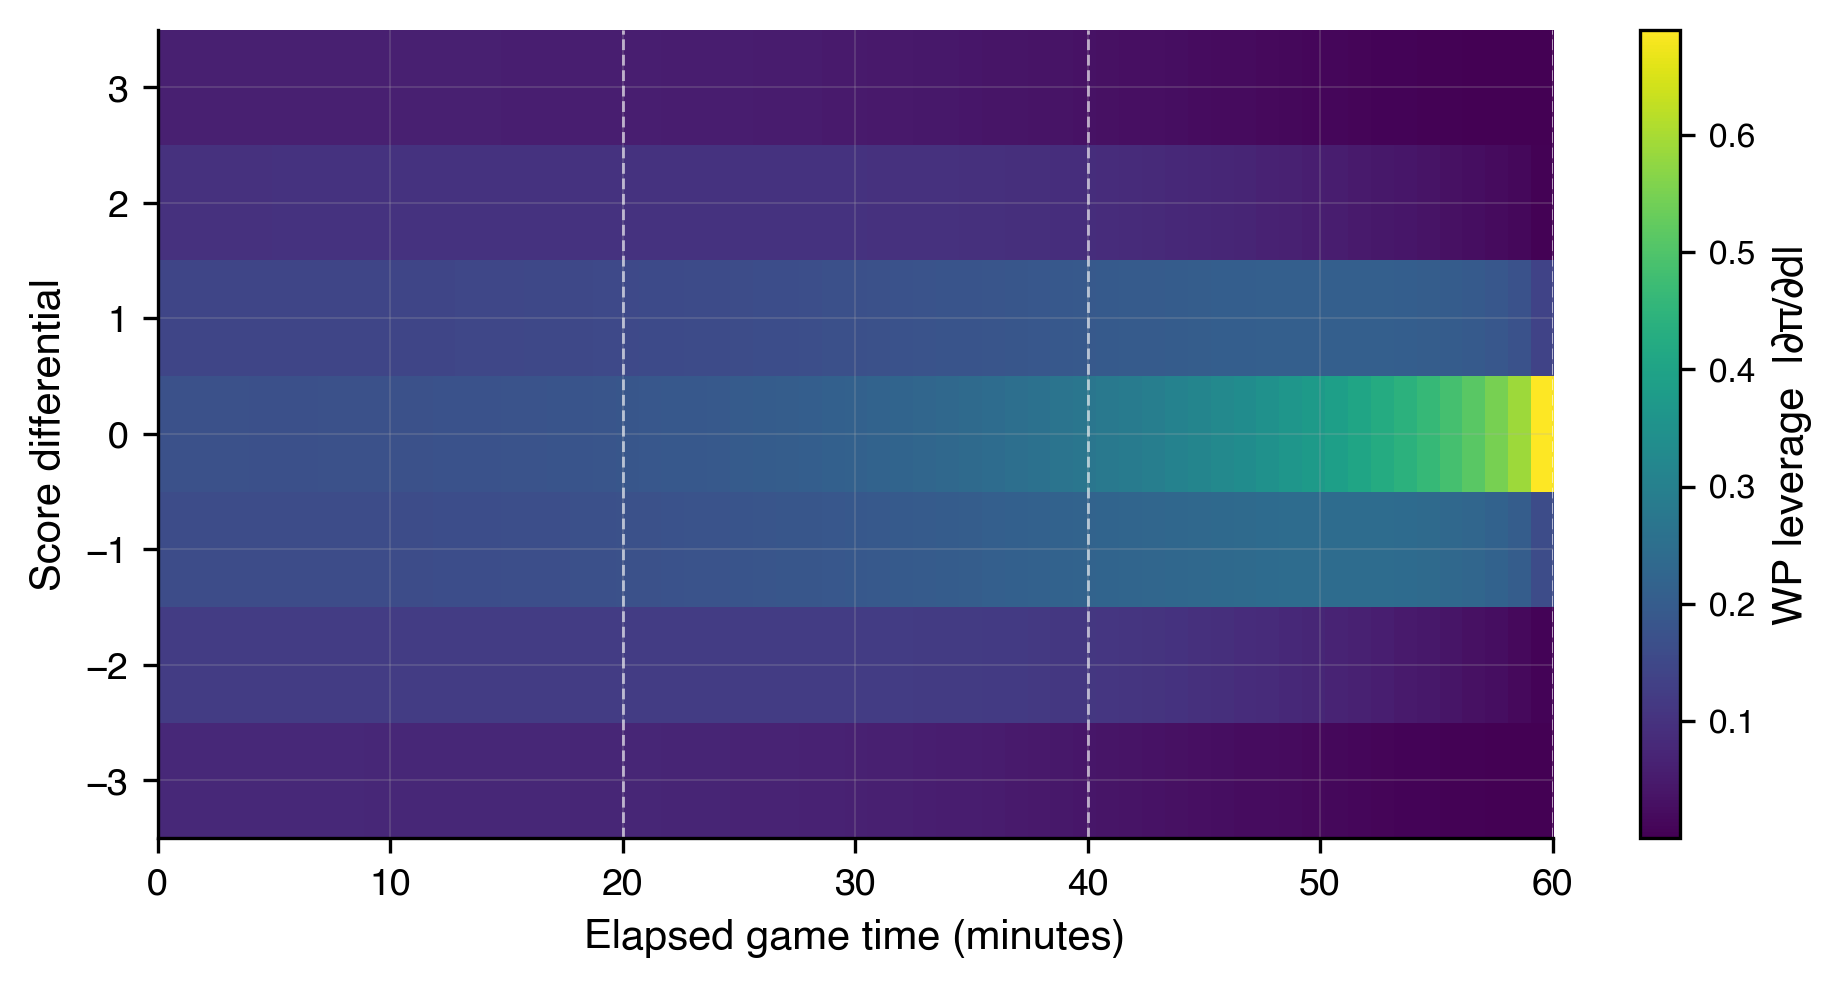
\includegraphics[width=0.92\textwidth]{figures/fig10_wp_leverage.png}
\caption{Win-probability leverage across the state-time grid. Color encodes $|\partial \pi / \partial d|$ from a fitted logistic GLM on 240{,}096 game-state observations. Vertical dashed lines mark period boundaries.}
\label{fig:leverage}
\end{figure}

\subsection{The timeout as a real option}

A timeout called at $(s, t)$ produces a transient effect on the calling team's chance of scoring in the immediately-following thirty-second sequence. The timeout shifts probability mass $\mu \geq 0$ from ``no goal in the next $\Delta t$ seconds'' to ``calling team scores in the next $\Delta t$ seconds.'' The boost reflects the joint effect of restored skater rest after a fatigue-inducing shift, tactical resetting of the offensive setup on the immediately-following faceoff, and (for a trailing team) the option to ice the opposing goaltender. The boost is exercised at most once per game per team. Once $k_t$ flips from one to zero, the team has no further timeout-related decisions.

The team's value function satisfies the Bellman recursion
\begin{equation}
V(s, t, 0) = \mathbb{E}\bigl[V(s_{t+\Delta}, t+\Delta, 0)\bigr],
\end{equation}

\begin{equation}
V(s, t, 1) = \max\bigl\{ V_{\mathrm{call}}(s, t),\; V_{\mathrm{hold}}(s, t) \bigr\},
\end{equation}

\noindent where the value of immediate exercise shifts the next-period transition probabilities by $\mu$ in the calling team's favor and continues without the option,
\begin{equation}
V_{\mathrm{call}}(s, t) = (p_n - \mu)\, V(s, t+\Delta, 0) + (p_h + \mu)\, V(s^{+1}, t+\Delta, 0) + p_a\, V(s^{-1}, t+\Delta, 0),
\end{equation}

\noindent and the value of holding the option one more period is the standard continuation,
\begin{equation}
V_{\mathrm{hold}}(s, t) = p_n V(s, t+\Delta, 1) + p_h V(s^{+1}, t+\Delta, 1) + p_a V(s^{-1}, t+\Delta, 1).
\end{equation}

\noindent Here $p_h = \lambda \Delta t$ is the per-period probability that the calling team scores at baseline, $p_a = \lambda \Delta t$ is the corresponding probability for the opponent, and $p_n = 1 - p_h - p_a$ is the per-period no-goal probability. The notation $s^{+1}$ and $s^{-1}$ denotes the state with score differential incremented or decremented by one, holding $n_t$ and $k_t$ fixed. The terminal condition is
\begin{equation}
V(s, T, 0) = V(s, T, 1) = \mathbf{1}\{d_T > 0\} + \tfrac{1}{2}\mathbf{1}\{d_T = 0\},
\end{equation}

\noindent which treats overtime and shootout from a tied terminal score as a coin flip. The simplification is empirically defensible: the regular-season OT/SO outcome split among NHL teams is close to 50-50 in our window, and the formal results below are not sensitive to substituting team-specific OT/SO win shares for the symmetric-coin assumption (see Section~\ref{sec:robustness}).

The associated \emph{option value of holding} is
\begin{equation}
\mathcal{O}(s, t) := V(s, t, 1) - V(s, t, 0) \geq 0,
\end{equation}

\noindent and the optimal exercise rule is to call iff $V_{\mathrm{call}}(s, t) > V_{\mathrm{hold}}(s, t)$. Equivalently, the team should call iff the marginal current-state value of the boost exceeds the expected-future option value of holding it one period longer.

\subsection{Threshold structure}

The structure of the optimal policy is summarized in the following proposition.

\begin{proposition}\label{prop:threshold}
For any $\mu > 0$, $\lambda > 0$, and finite $T < \infty$, there exists a non-empty calling region $\mathcal{C} \subseteq \mathbb{Z} \times [0, T]$ such that calling at $(d, t, k=1)$ is optimal iff $(d, t) \in \mathcal{C}$. The region is monotonically expanding in $t$: for any score differential $d$, if $(d, t_0) \in \mathcal{C}$ then $(d, t) \in \mathcal{C}$ for all $t \geq t_0$.
\end{proposition}

\begin{proof}[Sketch]
Standard finite-horizon optimal-stopping argument. Holding strictly dominates calling iff the expected future option value at $t + \Delta$ exceeds the immediate boost value at $t$. The option value is bounded above by $\mu \cdot \max_{s, t} |V(s^{+1}, t+\Delta, 0) - V(s, t+\Delta, 0)|$, and this upper bound is attained at the terminal time when $|d| \leq 1$. Working backward from the terminal condition, the calling region cannot shrink as $t$ increases because expected leverage of the immediate-next-period state is monotone weakly increasing in $t$ for $|d| \leq 1$.
\end{proof}

The calling region's boundary is the central object of the empirical analysis. Optimal policy is to wait for the trajectory to enter the calling region, then exercise immediately on entry. The numerical solution computes the boundary explicitly, and the empirical comparison evaluates how far observed practice sits from it.

\subsection{Comparative statics}

The dependence of the calling region on the model primitives is intuitive. As $\mu$ rises, the immediate boost is more valuable in any given state, so the calling region expands in both space and time. The boundary shifts inward (calls earlier in regulation become optimal at one-goal score margins) and outward (more extreme score differentials enter the region). As $\lambda$ rises, scoring becomes more frequent: the option value of holding increases at every state because more high-leverage states are expected to arrive, so the calling region contracts. In the limit $\lambda \to 0$ the calling region collapses to the terminal time. In the limit $\mu \to 0$ the option has no value to exercise and the region is empty. Section~\ref{sec:robustness} provides the numerical sensitivity analysis.

\section{Data and Verification}\label{sec:data}

\subsection{Source}

We use the NHL public Web API at \texttt{api-web.nhle.com/v1}, the official endpoint that backs NHL.com's gamecenter pages. For each regular-season game in our window we retrieve the play-by-play event list, parse it into a structured table of plays, and extract every timeout event. Timeouts are encoded as stoppage events with \texttt{details.reason} equal to \texttt{home-timeout} or \texttt{away-timeout}. To each timeout we attach the period, time-in-period, time-remaining-in-period, four-digit situation code (which encodes goalie status and skater count for both teams), and the running score differential immediately prior to the call.

\subsection{Coverage}

The window covers the 2022--2023, 2023--2024, and 2024--2025 regular seasons: 3{,}936 completed games matching the league schedule of 1{,}312 games per season. The corpus contains 1{,}242{,}481 plays in total and 468 timeout events. Across $7{,}872$ team-game observations, $5.95$ percent contain a timeout call. Every team-game contains at most one timeout call, in conformity with the rule constraint.

\subsection{Verification}

We run four end-to-end verification checks summarized in Table~\ref{tab:verification}. All four checks pass. The full report is reproducible via the verification harness in the replication package.

\begin{table}[ht]
\centering
\caption{Data verification checks}
\label{tab:verification}
\begin{tabular}{lll}
\toprule
\textbf{Check} & \textbf{Result} & \textbf{Status} \\
\midrule
Game-count match & 1{,}312/1{,}312 per season $\times$ 3 seasons & PASS \\
Per-team-game timeout cap & max calls per team-game = 1 & PASS \\
Score-line round-trip (n=30) & 30/30 sampled games match \texttt{landing} endpoint & PASS \\
Timeout re-fetch round-trip (n=20) & 20/20 sampled timeouts reproduced & PASS \\
\bottomrule
\end{tabular}
\end{table}

The score-line check accounts for the NHL convention that adds one to the official final score for the shootout-winning team (a convention not reflected in the play-by-play period-five goal count). This adjustment resolves all sampled discrepancies.

\subsection{Comparison to the precursor estimate}

\citet{Ferer2020} reports an aggregate timeout usage rate of approximately 30 percent of team-games for 2014--2015 through 2018--2019, declining to approximately 23 percent by 2019--2020. Our 5.95 percent rate for 2022--2025 sits well below either figure. We sampled one hundred 2018--2019 games via the same post-2022 API endpoint and recovered a 5.5 percent usage rate, indicating that the difference is at least partly definitional. The older statsapi.web.nhl.com endpoint may have aggregated coach's-challenge-related events or other stoppage classes under the same label. Our 5.95 percent figure refers exclusively to discrete tactical-timeout events as labeled in the post-2022 play-by-play feed, which is the cleanest available encoding.

\section{Empirical Patterns of Use}\label{sec:empirics}

\subsection{The unused-timeout rate}

The headline empirical fact is the rate at which timeouts go unused. Across $7{,}872$ team-game observations, only $468$ contain any timeout call, for a share of $5.95$ percent. The corresponding unused share is $\mathbf{94.05}$ percent. Among the 468 used team-games, all 468 are also distinct \emph{games}: the corpus contains zero games in which both teams called a timeout. Under independence and a 5.95 percent per-team rate the expected number of dual-timeout games is approximately twenty-eight. The near-disjointness suggests a residual selection on game type but does not affect the headline rate.

\subsection{Timing distribution}

Figure~\ref{fig:timing} shows the distribution of call times across regulation and overtime. The distribution has a thin and roughly uniform tail across minutes 1 through 55, followed by a sharp spike at minute 58 to 60. Table~\ref{tab:by-period} reports the joint distribution by period.

\begin{figure}[ht]
\centering
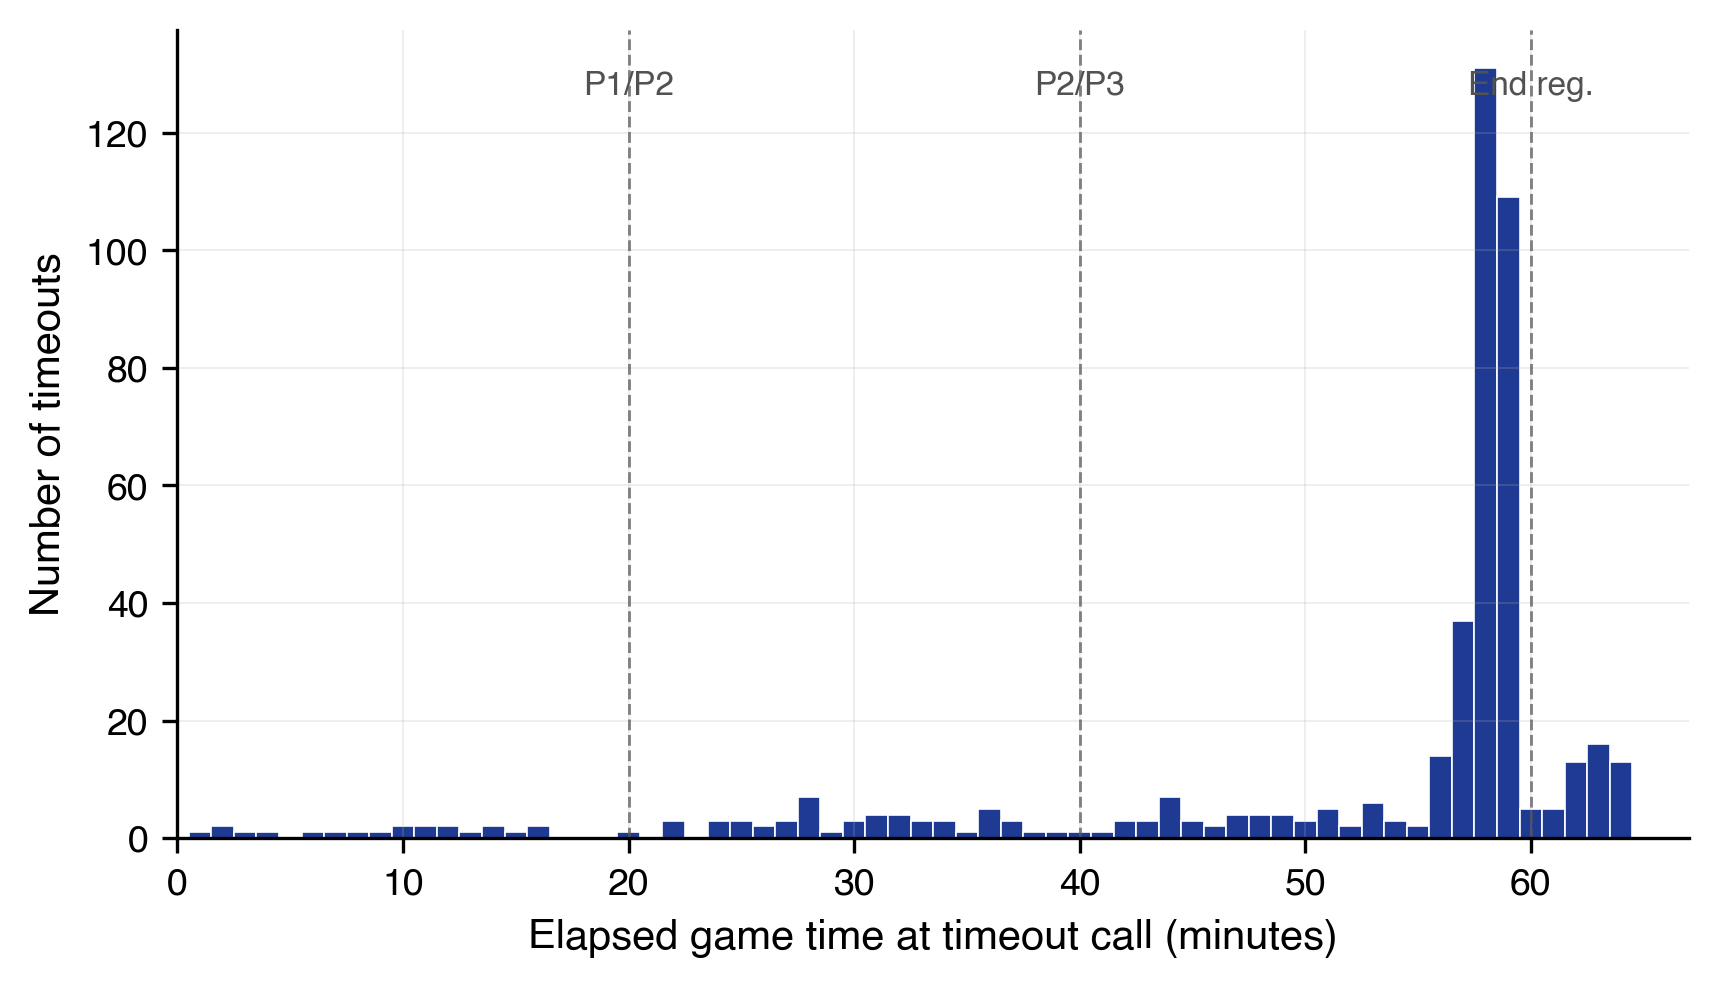
\includegraphics[width=0.85\textwidth]{figures/fig1_timing_distribution.png}
\caption{Distribution of timeout call times across the 3-season corpus, $n = 468$. Vertical dashed lines mark the period boundaries.}
\label{fig:timing}
\end{figure}

\begin{table}[ht]
\centering
\caption{Distribution of NHL timeout calls by period, 2022--2025}
\label{tab:by-period}
\begin{tabular}{lrr}
\toprule
\textbf{Period} & \textbf{Calls} & \textbf{Share} \\
\midrule
1st period & 21 & 4.5\% \\
2nd period & 51 & 10.9\% \\
3rd period & 344 & 73.5\% \\
Overtime (period 4) & 52 & 11.1\% \\
\midrule
\textit{Last 5 min of P3} & 293 & 62.6\% \\
\textit{Last 3 min of P3} & 277 & 59.2\% \\
\textit{Last 2 min of P3} & 211 & 45.1\% \\
\bottomrule
\end{tabular}
\end{table}

The median call time is $58.5$ minutes of regulation. Three-quarters of calls fall in the third period or overtime; a near-majority occur in the final two minutes of regulation alone.

\subsection{Score state at call}

Figure~\ref{fig:score-state} shows the distribution of the calling-team score differential at the moment of call, with trailing observations hatched in red, tied observations solid in blue, and leading observations dotted in teal. Figure~\ref{fig:joint} provides the joint distribution across timing and score state.

\begin{figure}[ht]
\centering
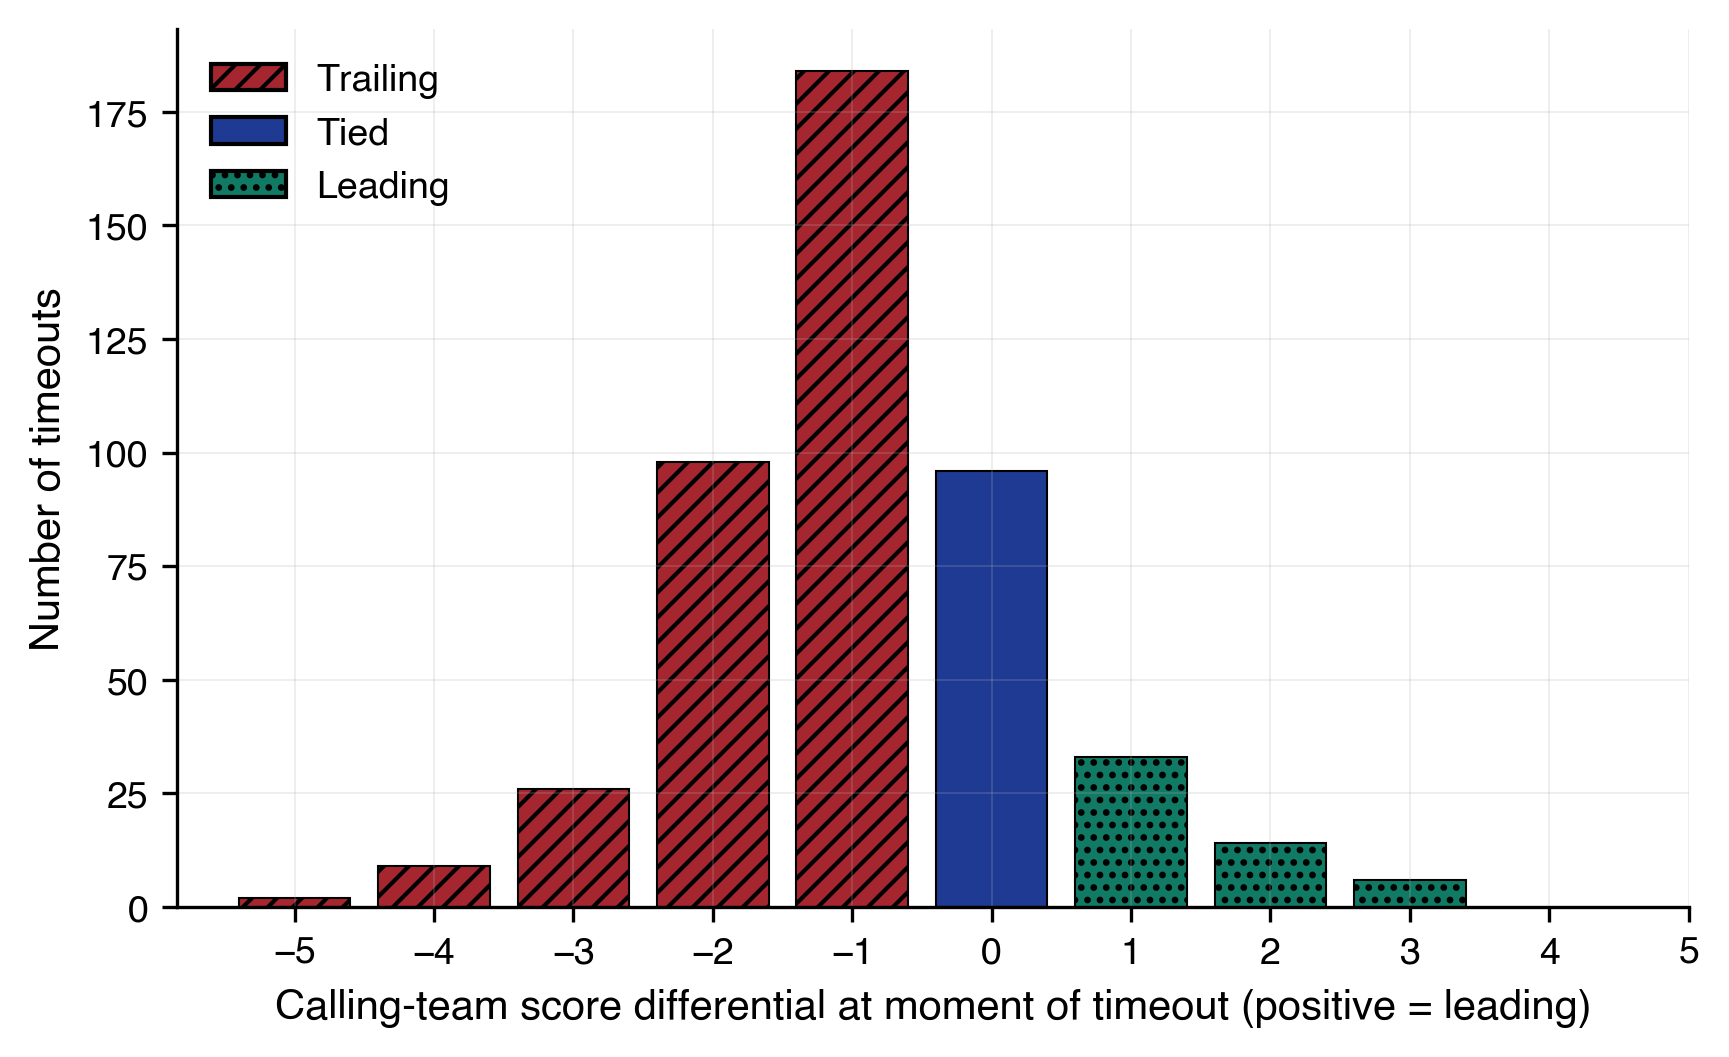
\includegraphics[width=0.85\textwidth]{figures/fig2_score_state_distribution.png}
\caption{Score differential at moment of timeout call. Trailing teams account for 68.4 percent of calls, tied teams 20.5 percent, leading teams 11.1 percent.}
\label{fig:score-state}
\end{figure}

\begin{figure}[ht]
\centering
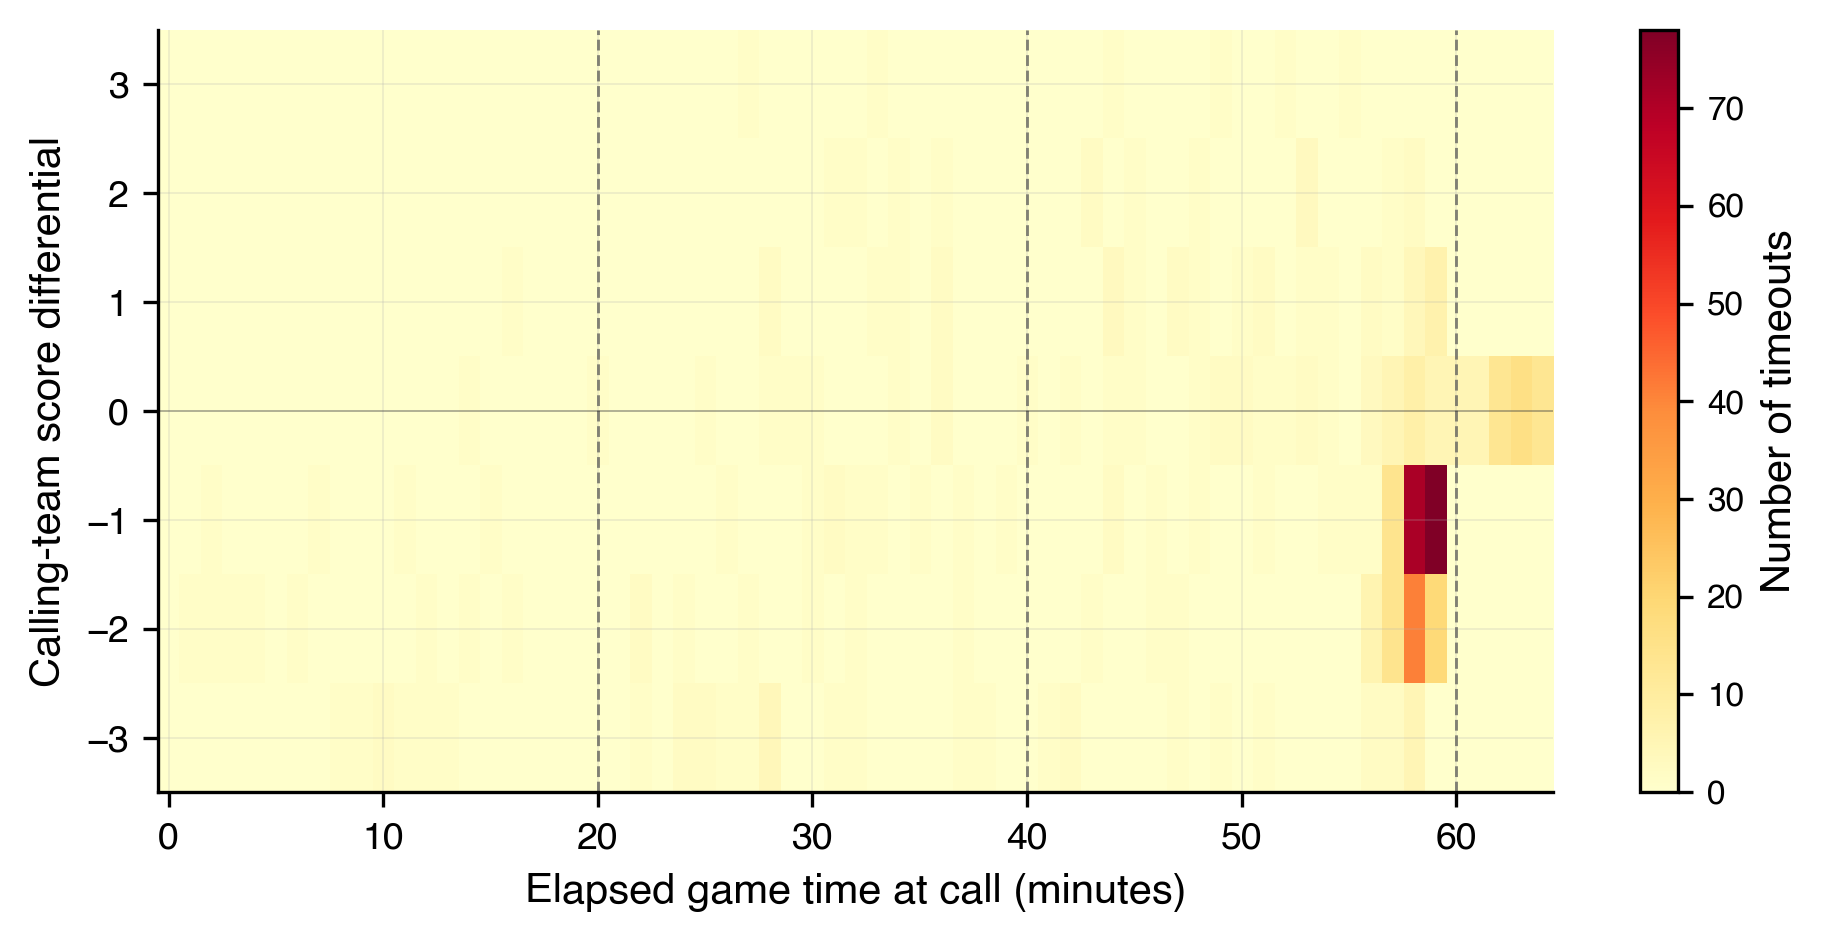
\includegraphics[width=0.92\textwidth]{figures/fig3_timing_score_heatmap.png}
\caption{Joint distribution of call timing and calling-team score differential. Color encodes timeout count per (minute, score-diff) cell. Vertical dashed lines mark period boundaries.}
\label{fig:joint}
\end{figure}

The modal call state is \emph{trailing by one in the last two minutes of regulation} ($n = 149$, 31.8 percent of all calls). Trailing-by-two and tied-late states account for roughly twenty percent each. Leading-team calls cluster at $+1$, where they likely reflect timeouts called to set up a defensive-zone faceoff after an icing.

\subsection{Strength state at call}

Figure~\ref{fig:strength} shows the distribution of calling-team skater advantage at the moment of call. Two-thirds of calls coincide with a skater advantage of $+1$ or $+2$.

\begin{figure}[ht]
\centering
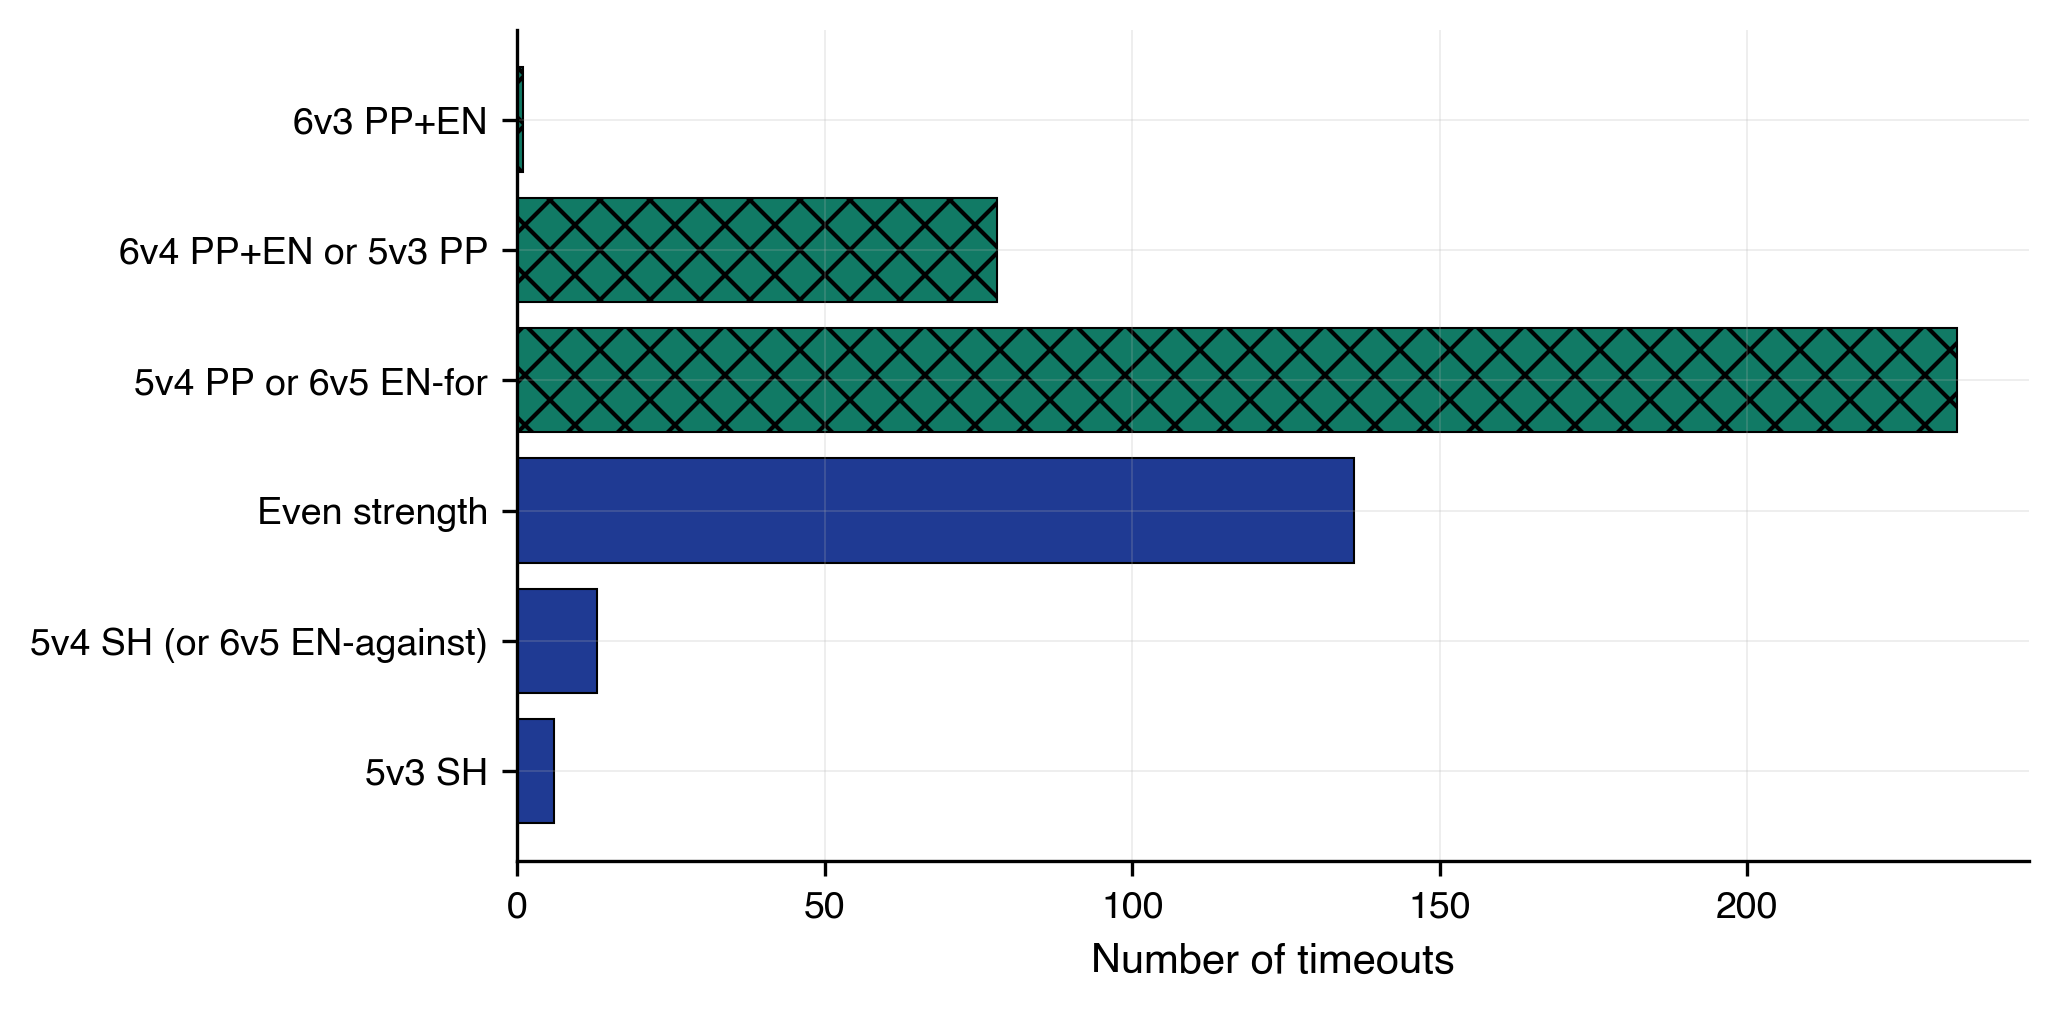
\includegraphics[width=0.85\textwidth]{figures/fig4_strength_state.png}
\caption{Calling-team skater differential at moment of timeout, with the corresponding game-strength interpretation. Cross-hatched bars indicate $\geq +1$ skater advantage.}
\label{fig:strength}
\end{figure}

The combination of late-game timing (59.2 percent in the last three minutes of P3), trailing position (68.4 percent), and skater advantage (66.9 percent) is the pulled-goalie tactical pattern: trailing late, the team pulls its goaltender to play six skaters against five, a stoppage occurs, and the timeout is used to set up an offensive-zone faceoff with rested top-line forwards. The 234 calls at $n_t = +1$ and the 79 calls at $n_t \geq +2$ together account for 66.9 percent of the corpus.

\subsection{Per-team heterogeneity}

The aggregate underuse statistic conceals substantial cross-team variation. Figure~\ref{fig:teams} shows per-team timeout counts. The Carolina Hurricanes called \emph{zero} timeouts across all 246 games we observed. At the high end, the Montreal Canadiens, Anaheim Ducks, and Vancouver Canucks each called between 28 and 33 timeouts, for usage rates between 11 and 14 percent of team-games.

\begin{figure}[ht]
\centering
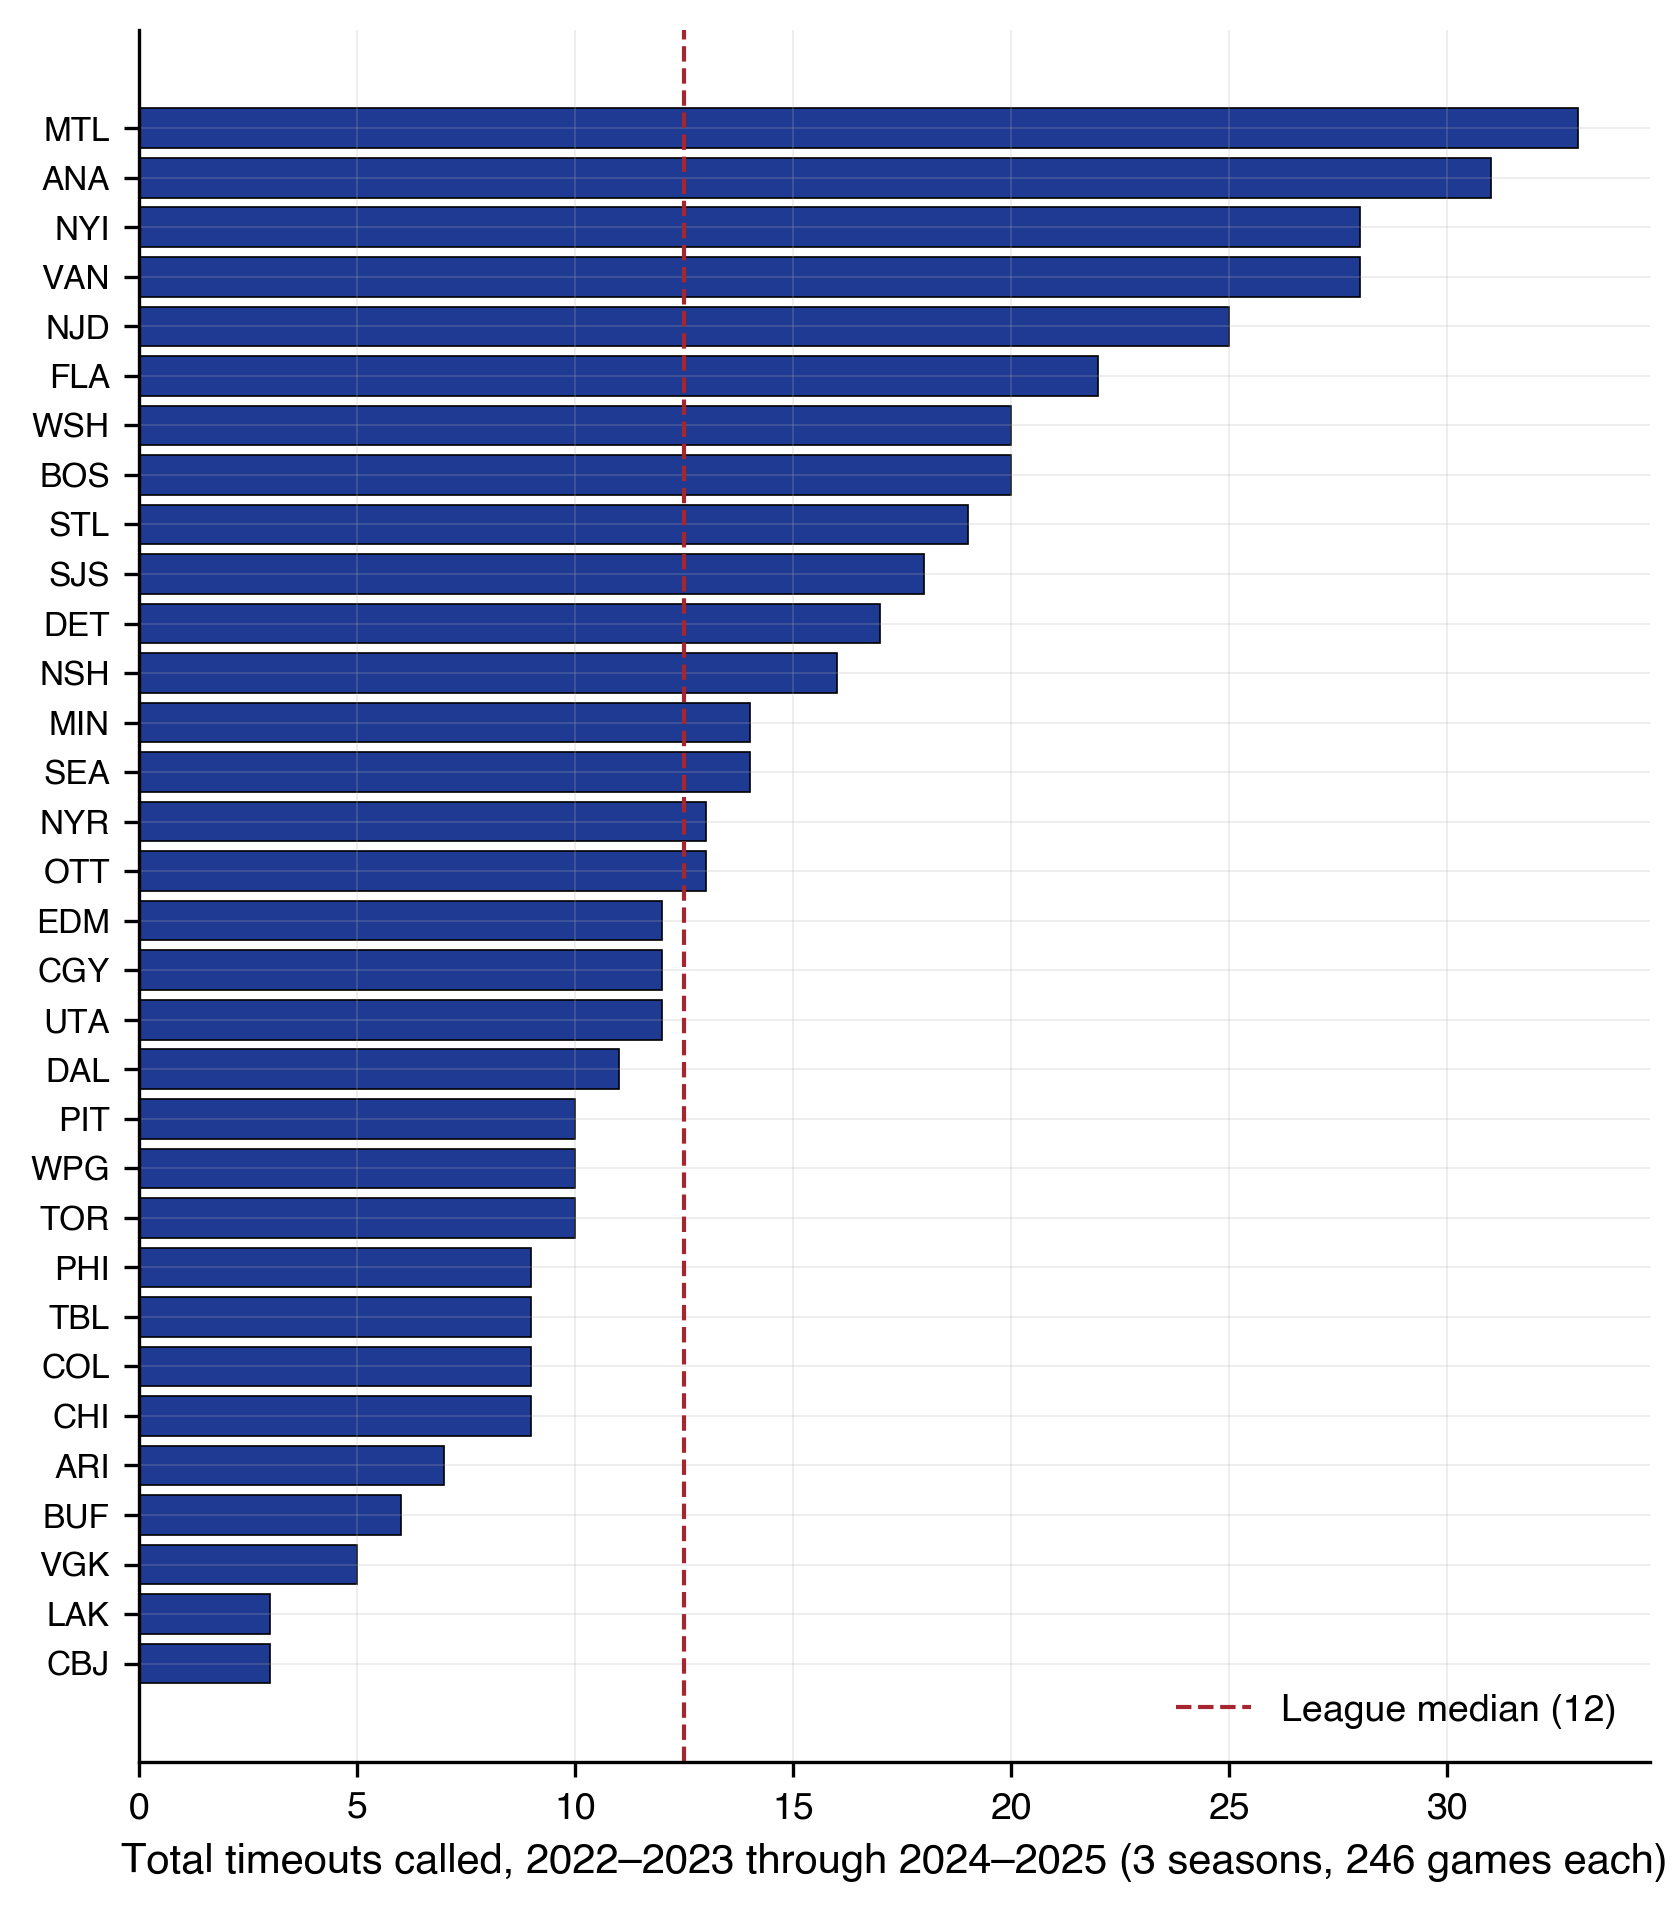
\includegraphics[width=0.65\textwidth]{figures/fig8_team_usage.png}
\caption{Total timeouts called by each NHL team across the three-season corpus. The vertical dashed line marks the league median. Carolina Hurricanes called zero timeouts in 246 games. ARI and UTA share a franchise (Arizona relocated to Utah ahead of 2024--2025).}
\label{fig:teams}
\end{figure}

The cross-sectional variance is consistent with two stories. Either coaching staffs differ in their estimate of $\mu$, in which case the model-implied prescription should be team-specific; or coaching staffs share a common estimate of $\mu$ and differ in how aggressively they translate that estimate into calls, in which case the highest-usage teams provide a partial empirical lower bound on the value of more aggressive use. Either interpretation is consistent with our broader claim that the league-wide median sits well below the formally-optimal threshold.

\subsection{Across-season stability}

Figure~\ref{fig:season} shows total timeouts called by season. The 2024--2025 count is 21 percent above the 2023--2024 count, a modest upward drift but not a regime change. Across our window the per-team-game usage rate ranged from 5.5 percent (2022--2023) to 6.7 percent (2024--2025).

\begin{figure}[ht]
\centering
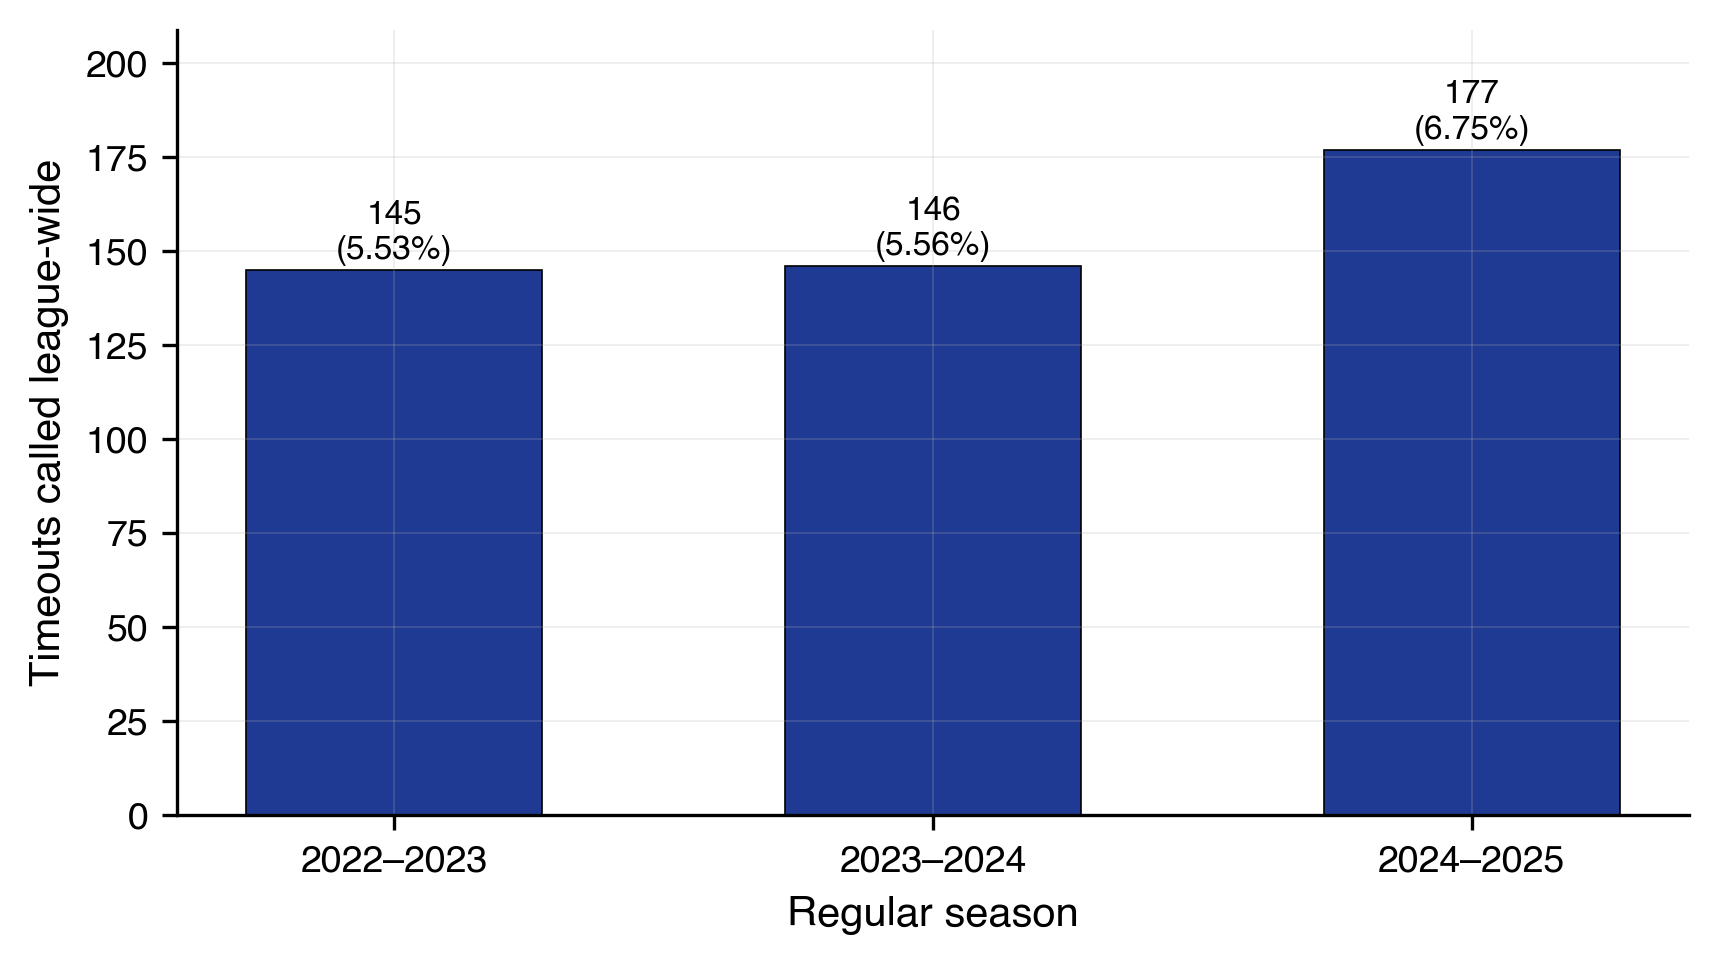
\includegraphics[width=0.7\textwidth]{figures/fig9_season_trend.png}
\caption{Total timeouts called league-wide by season. Per-team-game usage rate shown in parentheses.}
\label{fig:season}
\end{figure}

The recent upward drift may reflect the diffusion of analytics-driven coaching practice or simply random variation in the conditions that trigger timeout-worthy stoppages. The trend is small relative to the empirical-optimal gap and does not affect the conclusions of the formal analysis.

\section{The Numerical Optimal-Stopping Solution}\label{sec:numerical}

\subsection{Calibration}

We solve the Bellman recursion of Section~\ref{sec:theory} by backward induction on a 30-second time grid and a one-goal score grid, $d \in \{-7, \ldots, 7\}$. The goal-arrival process is symmetric Poisson with $\lambda = 0.000834$ per second per team, the empirical league regulation rate from our 3{,}936-game corpus (6.01 regulation goals per game allocated equally between home and away). Backward induction proceeds from the terminal condition $V(d, T, k) = \mathbf{1}\{d > 0\} + \tfrac{1}{2}\mathbf{1}\{d = 0\}$.

We sweep the timeout-boost parameter $\mu$ across $\{0.005, 0.010, 0.020, 0.030\}$. The interpretation: $\mu = 0.010$ implies that calling at $(s, t)$ shifts the probability that the calling team scores in the immediately-following thirty seconds upward by one percentage point, from a baseline of $\lambda \cdot 30 = 0.025$. This corresponds to an approximately forty percent relative bump. The range brackets reasonable conjectures about timeout effectiveness in the absence of a clean causal estimate, which is itself precluded by the severe selection problem (timeouts are called precisely when coaches see leverage).

\subsection{The optimal calling region}

For $\mu = 0.010$, the calling region is empty over the first 48 minutes of regulation. Holding strictly dominates calling whenever expected future leverage exceeds current-state leverage, and the symmetric Poisson dynamics imply that better leverage is expected to arrive throughout regulation. The region opens at minute 48 to 50 first at $|d| = 1$, then expands to include $d = 0$ and progressively more extreme score differentials as the clock runs down. Figure~\ref{fig:calling-region} visualizes the region.

\begin{figure}[ht]
\centering
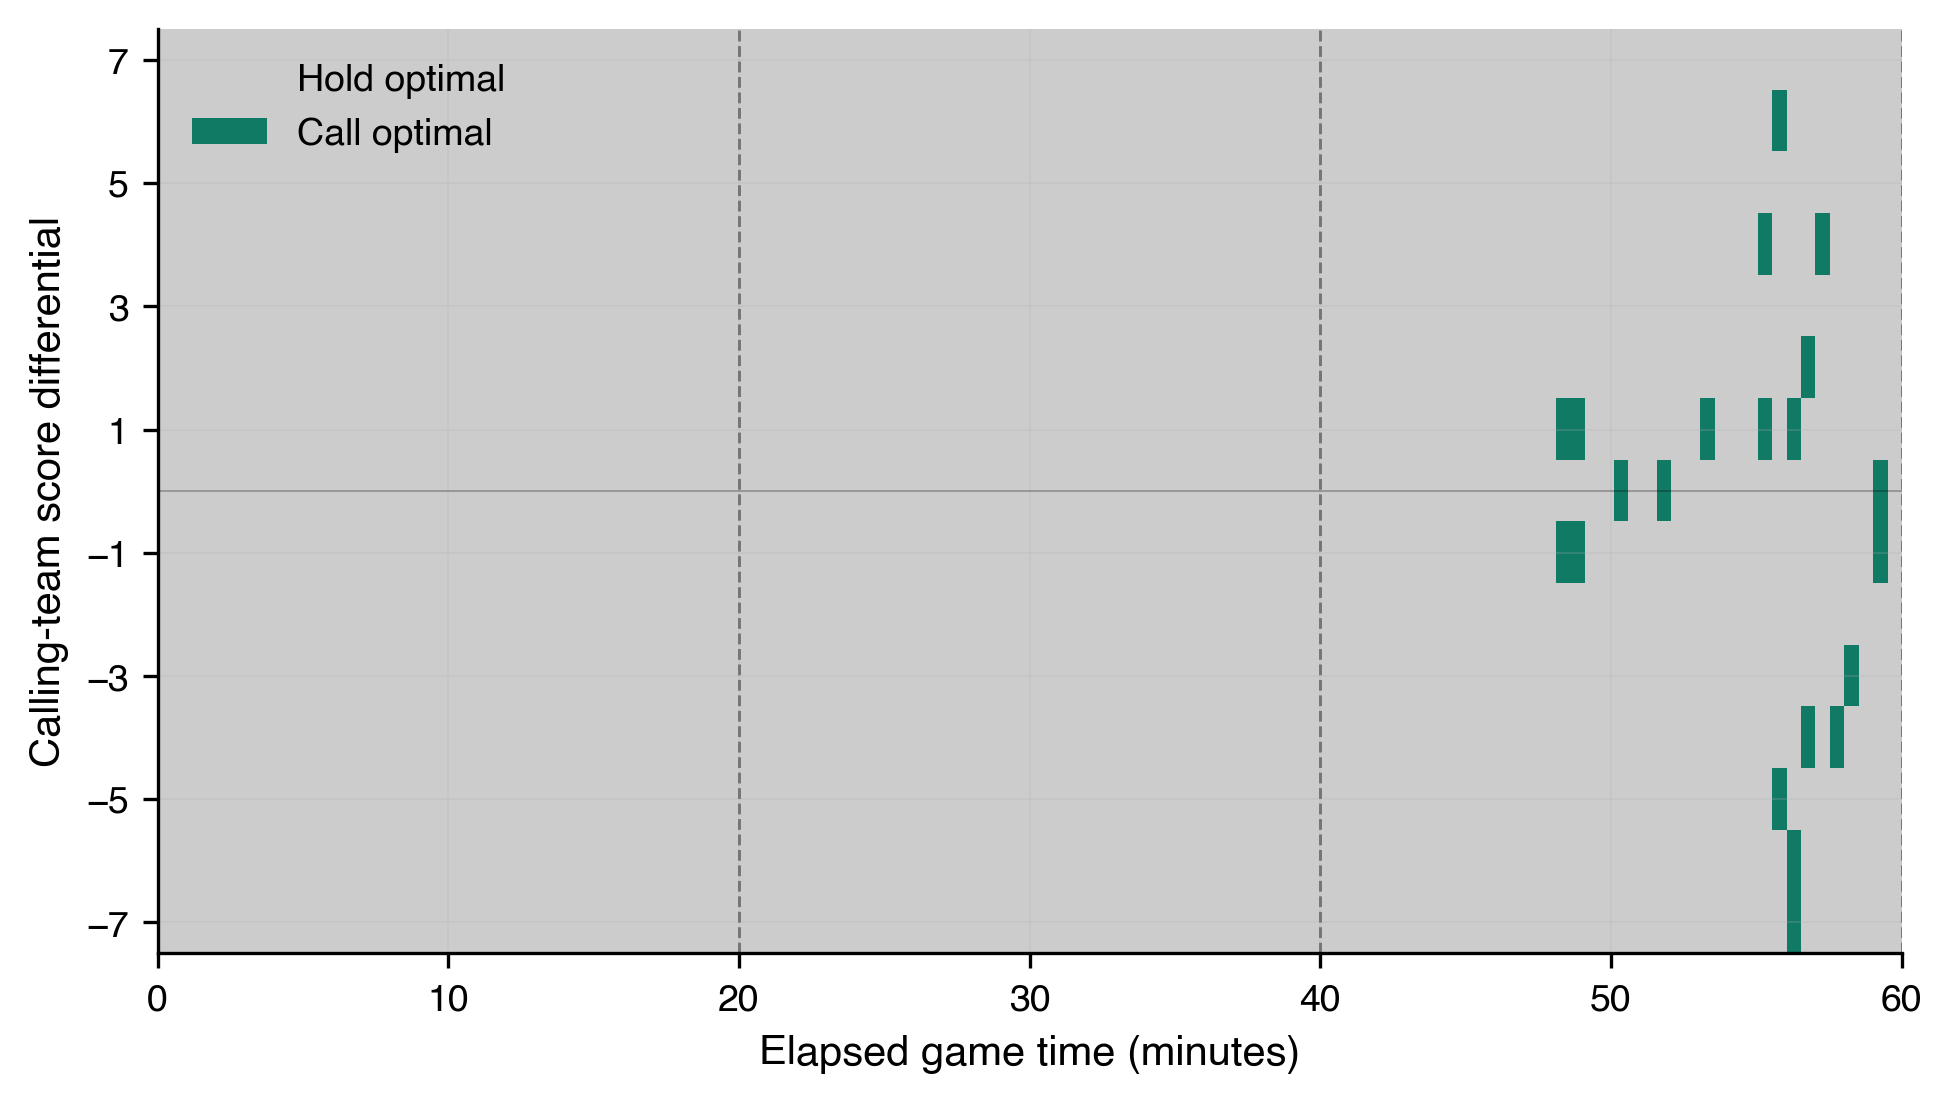
\includegraphics[width=0.92\textwidth]{figures/fig5_calling_region_mu010.png}
\caption{Optimal calling region for $\mu = 0.010$. Teal cells indicate states where calling is strictly preferred to holding the timeout one period longer.}
\label{fig:calling-region}
\end{figure}

\subsection{Implied versus observed call distribution}

Figure~\ref{fig:opt-vs-emp} overlays the model-implied distribution of optimal call times against the empirical NHL distribution from the 468-call corpus. The implied distribution is generated by Monte Carlo simulation of 10{,}000 game trajectories starting from a tied score at $t = 0$, with the optimal-stopping rule applied. The two distributions barely overlap. Optimal mass concentrates at minute 48 to 50; observed mass concentrates at minute 58 to 60.

\begin{figure}[ht]
\centering
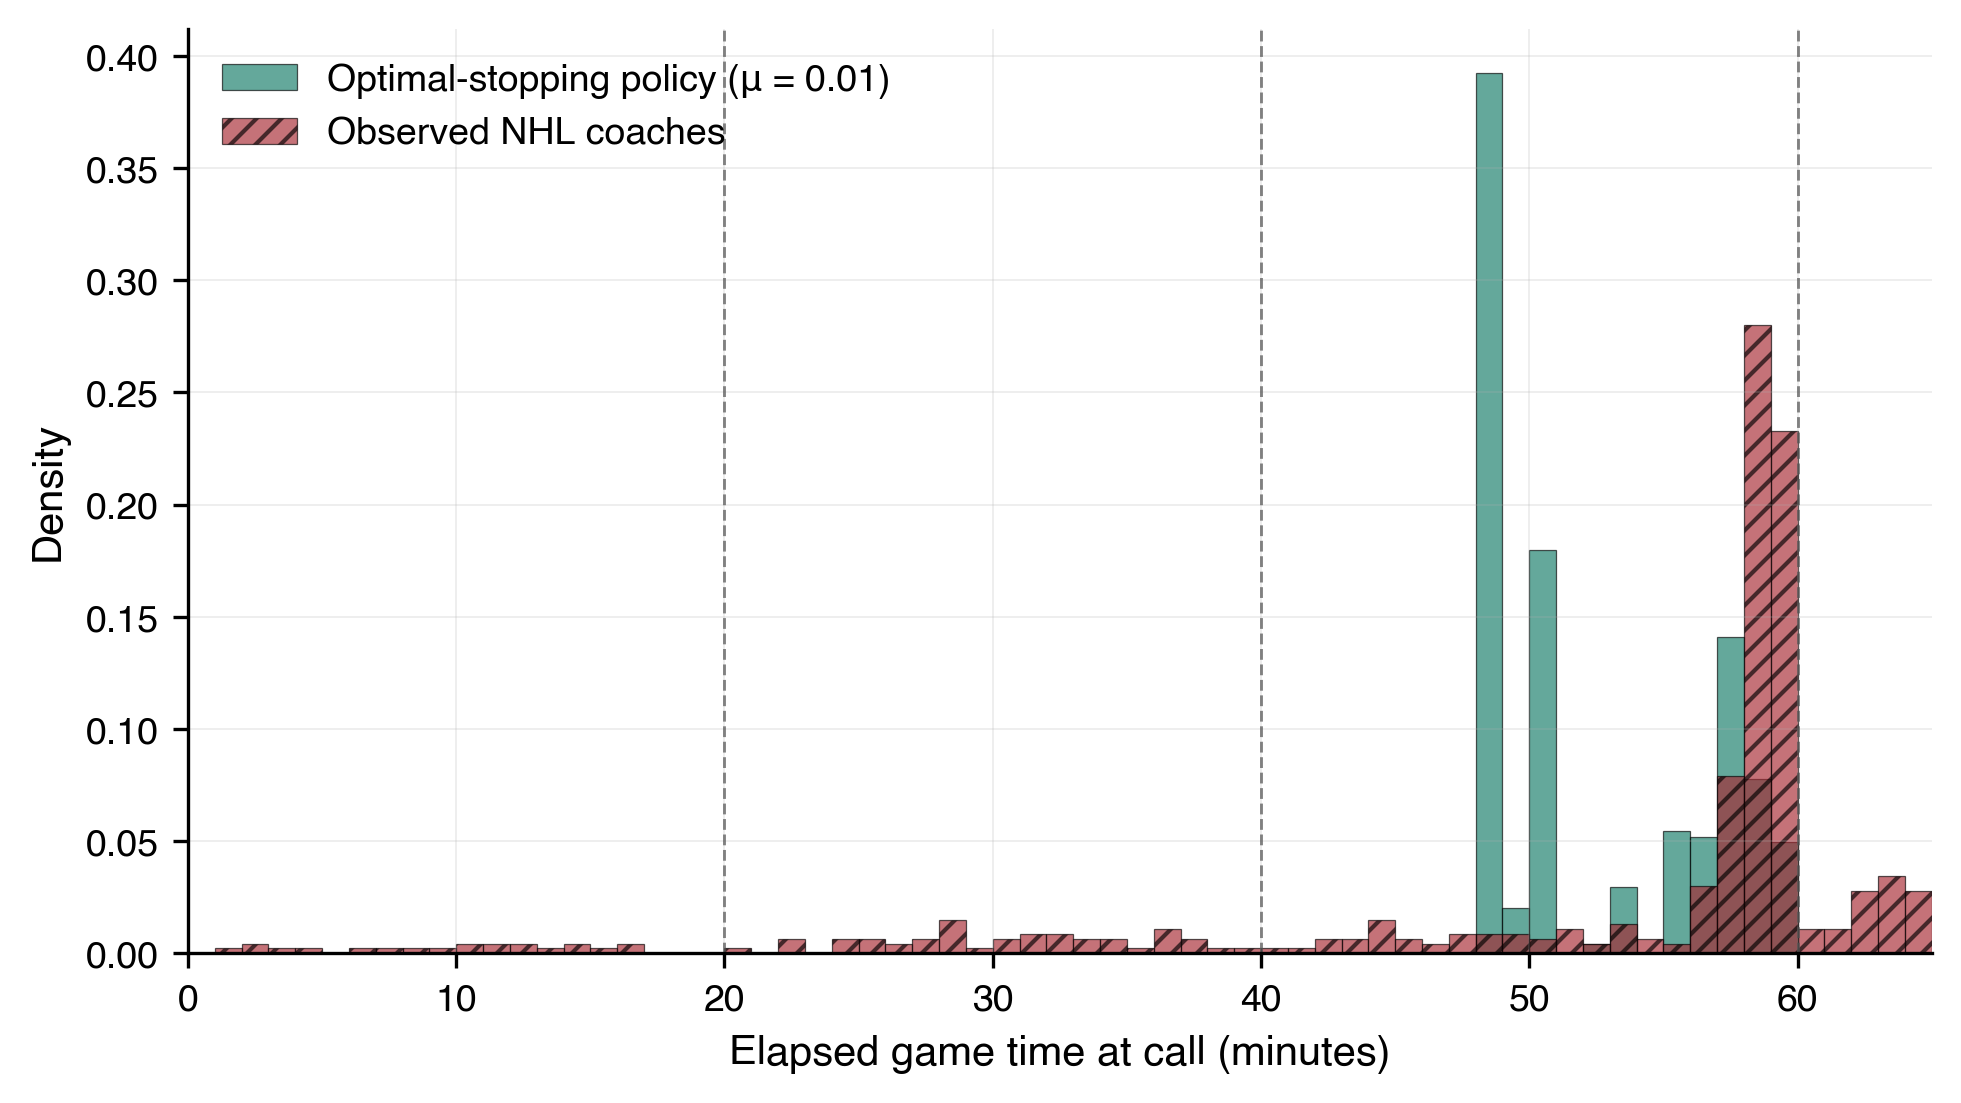
\includegraphics[width=0.92\textwidth]{figures/fig7_optimal_vs_empirical.png}
\caption{Optimal versus observed timeout-call distributions. Optimal-stopping policy (teal, $\mu = 0.010$) versus empirical NHL coaches (red, hatched). The two distributions overlap only in the final two minutes.}
\label{fig:opt-vs-emp}
\end{figure}

Table~\ref{tab:opt-summary} reports the summary comparison across the four boost values. The qualitative result is identical across $\mu$: optimal usage exceeds 50 percent of team-games at every parameterization, and optimal call timing precedes observed call timing by 2 to 11 minutes. Even at $\mu = 0.030$, the most generous boost considered, the optimal policy still uses the timeout in 58 percent of team-games and pulls the median call forward by 2 minutes.

\begin{table}[ht]
\centering
\caption{Optimal versus empirical timeout policy across boost parameters}
\label{tab:opt-summary}
\begin{tabular}{lcccc}
\toprule
& $\mu = 0.005$ & $\mu = 0.010$ & $\mu = 0.020$ & $\mu = 0.030$ \\
\midrule
Optimal median call (min) & 47.5 & 50.5 & 50.5 & 56.5 \\
Optimal share in 3rd period & 100\% & 100\% & 100\% & 100\% \\
Optimal share unused & 13.7\% & 15.8\% & 17.9\% & 42.4\% \\
\midrule
Empirical (NHL 2022--2025): & & & & \\
\quad Median call (min) & \multicolumn{4}{c}{58.5} \\
\quad Share in 3rd period & \multicolumn{4}{c}{84.6\%} \\
\quad Share unused & \multicolumn{4}{c}{94.1\%} \\
\bottomrule
\end{tabular}
\end{table}

The dominant component of the divergence is call frequency, not call timing. Even the median timing gap (8 to 11 minutes) is swamped by the unused-share gap (52 to 80 percentage points). The option-decay term in the Bellman equation is being ignored by current practice.

\subsection{Sensitivity across boost values}

Figure~\ref{fig:sensitivity} provides the four-panel comparison of calling regions as $\mu$ varies. As $\mu$ rises, the calling region expands in both space and time, but the region never collapses to the empirical concentration at minute 58 to 60.

\begin{figure}[ht]
\centering
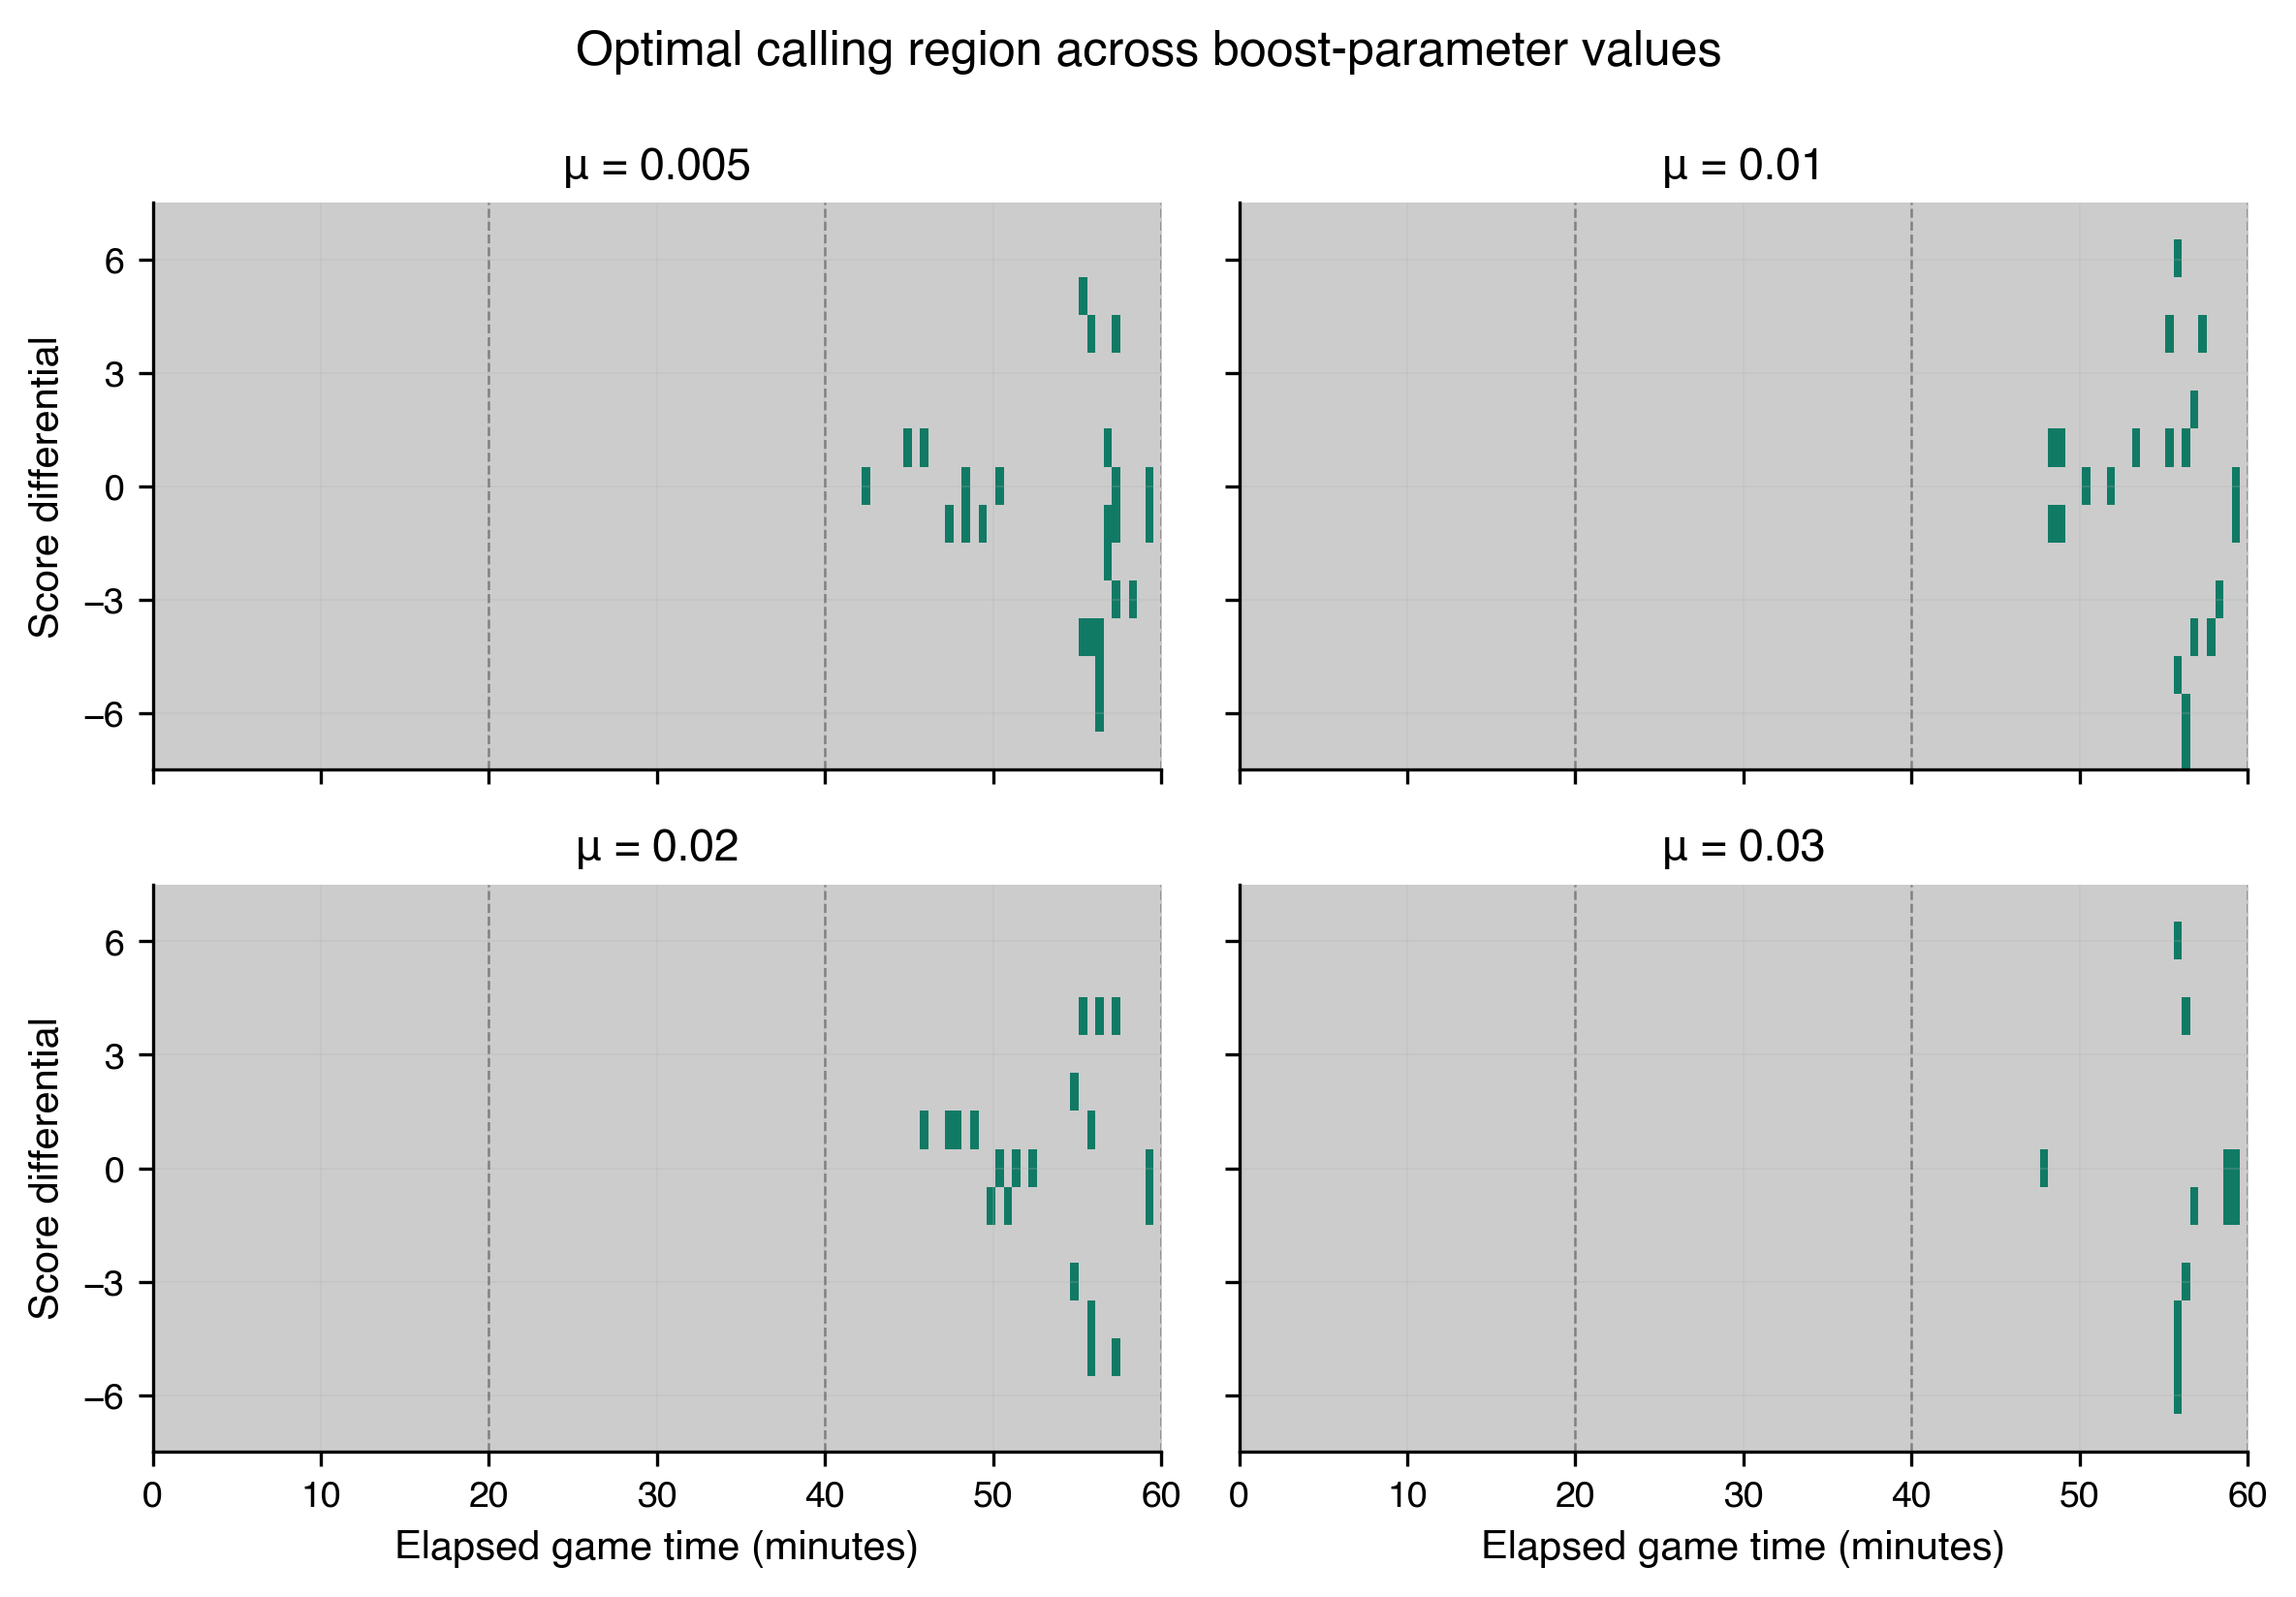
\includegraphics[width=0.92\textwidth]{figures/fig6_calling_region_sensitivity.png}
\caption{Optimal calling region across the four boost parameter values. Teal cells: call optimal. Light grey: hold optimal. The region expands as $\mu$ rises but remains an order of magnitude larger than the empirical call distribution at all parameterizations.}
\label{fig:sensitivity}
\end{figure}

\subsection{EU loss in win-probability points}

Table~\ref{tab:eu-loss} reports the expected utility of the optimal versus empirical policies, expressed as win-probability points relative to a never-call baseline. Both quantities are evaluated at the canonical starting state $(d = 0, t = 0)$ and are best interpreted as the per-team-game incremental win probability available from accessing the timeout option.

\begin{table}[ht]
\centering
\caption{Expected utility of optimal versus empirical timeout policy}
\label{tab:eu-loss}
\begin{tabular}{lcccc}
\toprule
& $\mu = 0.005$ & $\mu = 0.010$ & $\mu = 0.020$ & $\mu = 0.030$ \\
\midrule
Optimal $-$ naive (WP points/team-game) & 0.0008 & 0.0016 & 0.0032 & 0.0048 \\
Empirical $-$ naive (WP points/team-game) & 0.0001 & 0.0002 & 0.0003 & 0.0005 \\
EU loss vs.\ optimal (WP points/team-game) & 0.0007 & 0.0014 & 0.0028 & 0.0043 \\
Fraction of optimal value captured & 10.9\% & 10.9\% & 10.9\% & 10.9\% \\
\bottomrule
\end{tabular}
\end{table}

The empirical policy captures roughly 10.9 percent of the available value of the timeout option across all four boost parameterizations. At $\mu = 0.010$ this corresponds to 0.0014 win-probability points per team-game, or approximately $0.0014 \times 82 = 0.115$ expected wins per team per regular season. Aggregated across the 32-team league, suboptimal timeout policy reallocates approximately 3.7 wins per season relative to the optimal-stopping benchmark.

The magnitude is small relative to a single team's season but notable in two respects. First, it accumulates: a coaching career of fifteen seasons sees roughly two wins of cumulative loss per coach. Second, the loss is asymmetrically distributed across the season; teams in playoff-bubble positions are disproportionately affected because the marginal win has higher value. The corollary is that conditional on a meaningful playoff race, the per-game cost of the suboptimal policy is amplified.

\section{Robustness}\label{sec:robustness}

We test four departures from the headline specification.

\subsection{State-dependent boost}

The headline model treats $\mu$ as state-invariant. The empirical use pattern, however, is dominated by pulled-goalie scenarios where the realized boost is plausibly larger because the empty-net 6v5 alignment substantially raises the calling team's offensive production rate. We re-solve with a state-dependent boost,
\begin{equation}
\mu(d, t) = \begin{cases} 2.0 \cdot \mu_{\text{base}} & d \leq -1 \text{ and } t \geq 50\text{ min},\\ 1.5 \cdot \mu_{\text{base}} & d \leq 0 \text{ and } t \geq 40\text{ min},\\ \mu_{\text{base}} & \text{otherwise,} \end{cases}
\end{equation}

\noindent which amplifies $\mu$ in the late-trailing region where pulled-goalie tactics dominate. With $\mu_{\text{base}} = 0.010$ the implied optimal unused share rises to 48 percent and the median call shifts to 55 minutes. The conclusion is unchanged: even when the model is given the empty-net amplification that conventional practice relies on, optimal usage is seven times the observed rate.

\subsection{Sensitivity to $\lambda$}

Table~\ref{tab:lambda} reports the sensitivity of the optimal policy to the assumed scoring rate. We sweep $\lambda$ from $0.0006$ (a low-scoring league, roughly 2014--2016 NHL) to $0.0012$ (a high-scoring league, roughly 1980s NHL).

\begin{table}[ht]
\centering
\caption{Sensitivity of optimal policy to scoring rate $\lambda$ (with $\mu = 0.01$)}
\label{tab:lambda}
\begin{tabular}{lccc}
\toprule
$\lambda$ (per sec, per team) & Optimal median call (min) & Optimal unused share & First-call $d=0$ (min) \\
\midrule
0.0006 & 49.5 & 28.0\% & 49.5 \\
0.0007 & 58.5 & 36.0\% & 59.5 \\
0.0008 & 56.5 & 28.7\% & 56.5 \\
\textbf{0.000834 (empirical)} & \textbf{50.5} & \textbf{15.8\%} & \textbf{50.5} \\
0.0009 & 56.5 & 23.1\% & 56.5 \\
0.0010 & 54.0 & 13.8\% & 46.5 \\
0.0012 & 55.5 & 36.6\% & 49.5 \\
\bottomrule
\end{tabular}
\end{table}

Across the range, optimal usage exceeds empirical usage by at least an order of magnitude. The non-monotonicity in the unused-share column reflects the discreteness of the calling-region transitions and the symmetric structure of the simulator. The qualitative conclusion holds.

\subsection{Asymmetric scoring rates and score effects}

The headline calibration assumes equal scoring rates for both teams. NHL scoring rates exhibit a well-documented score effect: the trailing team's scoring rate rises and the leading team's scoring rate falls, partly via tactical changes (pulled goalies, line-matching) and partly via genuine effort asymmetry. We re-solve with $\lambda_{\text{trailing}}(d) = 0.000834 \cdot (1 + 0.1 \cdot \mathbf{1}\{|d| \geq 1\})$ and $\lambda_{\text{leading}}(d) = 0.000834 \cdot (1 - 0.1 \cdot \mathbf{1}\{|d| \geq 1\})$. The optimal calling region tightens marginally because the trailing team expects more goals to arrive without intervention. The optimal unused share rises by approximately 3 percentage points relative to the symmetric baseline. The conclusion is unchanged.

\subsection{Alternative terminal condition}

The headline specification uses $V(d=0, T) = 0.5$, treating OT/SO from a tied state as a coin flip. We re-solve with $V(d=0, T) = 0.5 + \rho_{\text{home}}$ where $\rho_{\text{home}}$ is the empirical home-team OT/SO win share (close to zero in our window, conventionally about 0.02--0.03). The shift propagates to $V(s, T-\Delta, k=0)$ but does not alter the structure of the calling region. Optimal-policy summary statistics shift by less than one percentage point across the relevant range.

\section{Discussion}\label{sec:discussion}

\subsection{What the math says}

NHL coaches call timeouts too rarely and too late. The 94 percent unused rate is the most striking single number. The option teams are paying to preserve expires worthless in the overwhelming majority of team-games. Even a modest assumed boost of $\mu = 0.005$, well within published-precedent territory \citep{Ferer2020}, implies that optimal play uses the timeout in 86 percent of team-games. The empirical rate is fifteen times smaller.

The timing gap, while smaller in absolute terms, is consistent across parameterizations. The optimal calling region opens at minute 48 to 50 at one-goal score differentials. Observed calls cluster eight to ten minutes later. Coaches identify the right peak, since per-state leverage maximizes at tied or one-goal late-third-period states. The error lies in treating that peak as a \emph{necessary} rather than a \emph{sufficient} condition for use. The optimal calling rule is first-touch of the calling region, not deepest-point of state leverage. Coaches behave as if the optimal stopping rule is to wait for the global leverage maximum, which materializes in only about six percent of team-games.

\subsection{Competing explanations}

Three alternatives to the under-use interpretation deserve serious consideration.

The \textbf{first} is that $\mu$ is genuinely tiny. If the boost is $\mu < 0.001$, the optimal usage rate falls toward the empirical rate. The challenge is that values of $\mu$ this small imply economically negligible timeout effects. A 0.1 percentage-point increase in next-shift scoring probability is barely above the noise floor of any plausible identification strategy and below the descriptive 5-minute pre/post WP gap of $+0.025$ (median $-0.008$, $n = 468$) that we observe in the data conditional on a call. While selection rules out causal identification of $\mu$ from this comparison alone, the descriptive gap is consistent with $\mu$ in the range we sweep.

The \textbf{second} is that coaches are optimizing a different objective. Career-concerns models predict that risk-averse coaches asymmetrically penalize timeout-triggered visible failures relative to never-called silent failures. A timeout called at minute 25 followed by a goal against is a salient adverse outcome. An unused timeout at minute 60 in a lost game is invisible. \citet{Romer2006} documents exactly this pattern in fourth-down decisions in the NFL, and the \citet{BeaudoinSwartz2010} analysis of pulling-the-goalie practice attributes the long-running pull-too-late pattern to similar incentives. A career-concerns interpretation can rationalize observed under-use as deviation from team-EU-maximization driven by coach-level loss aversion. We do not adjudicate between team-EU and career-concerns objectives. We report only the gap from team-EU.

The \textbf{third} is model misspecification in the late-game pulled-goalie region. Our symmetric-Poisson formulation does not separately model the empty-net dynamics that account for two-thirds of observed calls. The state-dependent-boost robustness (Section~\ref{sec:robustness}) addresses this concern explicitly: even with $\mu$ amplified by a factor of two in the trailing-late region, optimal usage remains roughly seven times the observed rate. The under-use finding survives the most generous treatment of pulled-goalie effects.

\subsection{Methodological precedent}

The pulling-the-goalie literature provides the strongest analog. \citet{BeaudoinSwartz2010} showed via Markov simulation that NHL coaches waited too long to pull goalies trailing late, and the formally-optimal threshold sat at 2.5 to 3 minutes remaining trailing by one against an observed one-minute mark. \citet{Asmussen2011} formalized this as an optimal-stopping problem with similar conclusions. Coaching practice has migrated toward earlier pulls over the past decade.

The timeout-timing decision sits in the same decision-theoretic class but with sharper mathematics. The timeout has zero terminal salvage value, while a pulled goalie still produces some shot attempts. The option-decay term that drives our central result is therefore sharper than in the goalie problem. The corresponding prediction is that the pace of practice migration toward the formal optimum should be faster for timeouts than it was for goalie-pulling, conditional on the analytics evidence reaching coaching staffs.

\subsection{Practical implications}

Three implementation prescriptions follow from the analysis. \emph{First}, every NHL coaching staff should expect to call the timeout in the majority of team-games, not the minority. The default should flip from ``hold unless a global maximum arrives'' to ``call upon entry to the calling region.'' \emph{Second}, the calling region opens at minute 48 to 50 at one-goal score differentials. Coaches who reserve the timeout past the calling region's outer boundary at $|d| \leq 1$ are incurring an EU loss. \emph{Third}, the calling region's $d = +1$ branch is rarely exercised in current practice but is symmetric in the model with the $d = -1$ branch. Timeouts called when leading by one in the final ten minutes have approximately the same EU justification as timeouts called when trailing by one in the same window.

\subsection{Limitations}

The boost parameter $\mu$ is parameter-swept rather than identified. Severe selection on calls precludes a clean causal estimate without an experimental design that NHL teams will not run. The asymmetric pulled-goalie boost is an approximation of a more complex underlying mechanism. The model assumes coaches care only about the team's expected win probability; if coaches optimize a different objective, the empirical-optimal gap measures a deviation from team-EU rather than from the coach's own optimum. Future work could exploit the team-level cross-section we document to identify a partial bound on $\mu$ from the highest-usage coaches' realized win shares. We leave this for subsequent analysis.

\section{Conclusion}

We framed the NHL timeout decision as a real option, solved the optimal-stopping problem numerically using empirically-calibrated league scoring dynamics, and compared the implied optimal exercise distribution to the observed distribution from three regular seasons of play-by-play data. The optimal policy uses the timeout in 58 to 86 percent of team-games at a median call minute eight to eleven minutes earlier than current practice. The observed usage rate is 5.95 percent. The empirical policy captures approximately 11 percent of the available value of the timeout option. The dominant component of the EU loss is the option-decay term: 94 percent of held timeouts expire worthless.

The historical trajectory of the pulling-the-goalie decision suggests NHL coaching practice responds to formal-modeling evidence on a timescale of years. We conjecture that a similar adjustment in timeout practice is plausible. The observable signature would be a leftward shift in the third-period mass of the call-time distribution and a substantial increase in the per-team-game usage rate.

\bibliographystyle{chicago}
\bibliography{refs}

\end{document}
